% !TEX root =thesis.tex
% !TEX root =thesis.tex
%---------------------------------------------------------------------------
% Vorlage für Bachelorarbeiten, Masterarbeiten
% der AG Autonome Intelligente Systeme
% Basierend auf der Vorlage der AG PRIA an der Universität Münster
% (Autoren dort: Daniel Tenbrinck, Fabian Gigengack, Michael Schmeing, Lucas Franek, Andreas Nienkötter
% Dazu Dank an Phil Steinhorst und dessen Vorlage, von der Teile übernommen wurden
%---------------------------------------------------------------------------

\documentclass[%
  paper=A4,               % Papiergröße
  twoside=true,           % zweiseitiges Layout
  openright,              % Kapitel auf ungerader Seite beginnen
  11pt,                   % Schriftgröße
  bibliography=totoc,     % Literaturverzeichnis im Inhaltsverzeichnis
  %listof=totoc,           % Abb.-/Tab.-verzeichnis im Inhaltsverzeichnis
  titlepage=on,           % Titel auf eigener Seite
  DIV=12,                 % Satzspiegelberechnung
  BCOR=1.5cm,             % Bindungskorrektur
  parskip=half,           % Absatzabstand
  final
]{scrreprt}

% Basics
\usepackage[x11names]{xcolor}

\usepackage{natbib}

% Schriftarten setzen
\usepackage[T1]{fontenc}
%\usepackage[utf8]{inputenc} % UTF-8 Codierung
\usepackage{microtype}
\usepackage{charter}
\usepackage{sourcesanspro}
\usepackage{nimbusmononarrow}
%\renewcommand*\familydefault{\sfdefault}   % aktivieren für serifenlose Schrift

\usepackage{array}
\usepackage{booktabs}\newcommand{\ra}[1]{\renewcommand{\arraystretch}{#1}}
\usepackage{adjustbox}

% Absatzformatierung
\usepackage{setspace}
\onehalfspacing
\setlength{\parindent}{0cm}

% Sprachoptionen
%\usepackage[ngerman]{babel}
\usepackage[english]{babel}
%\usepackage[german=quotes]{csquotes}    % passende Anführungszeichen

% Kopf- und Fußzeile
\usepackage[headsepline=1pt, automark]{scrlayer-scrpage}
\setkomafont{pageheadfoot}{\sffamily}       % Kopfzeile serifenlos
\setkomafont{pagenumber}{\sffamily\Large}   % Seitenzahl serifenlos und etwas größer
\setkomafont{headsepline}{\color{gray}} % adds a gray line under the header
\renewcommand*{\footfont}{\sffamily\color{gray}}

% adds a thick gray line after the chapter number
\renewcommand*{\chapterformat}{%
    \thechapter\enskip
    \textcolor{gray!50}{\rule[-\dp\strutbox]{1.5pt}{\baselineskip}}\enskip
}

% Alles rund um Floats
\usepackage{graphicx}
\usepackage{subfigure} % Um mehrere Bilder in eine figure einzufügen

% Mathe-Pakete
\usepackage{mathtools}
\usepackage{amsthm}
\usepackage{amssymb}
\usepackage{thmtools}

% Colored tables are fancy
\usepackage[table]{xcolor}
\usepackage{colortbl}

% fancy prompts
\usepackage{caption}

\DeclareCaptionLabelFormat{prompt}{Prompt #2}

% Definition der Styles für mathematische Definitionen, Sätze, Beweise, etc.
\declaretheoremstyle[                     % Style für Definitionen, Sätze, Behauptungen, etc.
  headfont=\sffamily\bfseries,            % Font für Überschrift
  notefont=\normalfont\sffamily\itshape,  % Font für Bezeichnung in Klammern
  bodyfont=\normalfont,                   % Font für Inhalt
  headformat=\NAME\ \NUMBER\; \NOTE,      % Reihenfolge: Erst Definition/Satz/etc., dann Nummer, dann Bezeichnung
  headpunct={},                           % kein Punkt am Ende der Überschrift
  postheadspace=\newline,                 % Zeilenumbruch nach Überschrift
  mdframed={                              % Gestaltungsoptionen
    skipabove=1em,
    skipbelow=1em,
    innerleftmargin=1em,
    innerrightmargin=1em,
    hidealllines=true,
    backgroundcolor=gray!15
  },
]{mainstyle}

\declaretheoremstyle[             % Style für Beweise
  headfont=\bfseries\scshape,
  bodyfont=\normalfont,
  headpunct=:,
  postheadspace=2em,
  qed=\qedsymbol
]{proofstyle}

% Definition der entsprechenden Umgebungen
\declaretheorem[                  % Umgebung für Definitionen
  name=Definition,                % auszugebender Name
  parent=chapter,                 % Nummerierung mit vorgestellter Kapitelnummer
  style=mainstyle                 % Nutze mainstyle-Definition (siehe oben)
]{definition}                     % Name der Umgebung

\declaretheorem[                  % Umgebung für Sätze
  name=Satz,
  sharenumber=definition,         % gemeinsame Nummerierung mit definition
  style=mainstyle
]{satz}

\declaretheorem[                  % Umgebung für Beweise
  name=Beweis,
  numbered=no,                    % Beweise sind nicht nummeriert
  style=proofstyle
]{beweis}

% -- Definition der einzelnen Umgebungen
\declaretheoremstyle[%
  headfont=\sffamily\bfseries,
  notefont=\normalfont\sffamily,
  bodyfont=\normalfont,
  headformat=\NAME\ \NUMBER\NOTE,
  headpunct=,
  postheadspace=\newline,
  spaceabove=\parsep,spacebelow=\parsep,
  %shaded={bgcolor=gray!20},
  postheadhook=\theorembookmark,
  mdframed={
    backgroundcolor=gray!20,
    linecolor=gray!20,
    innertopmargin=6pt,
    roundcorner=5pt,
    innerbottommargin=6pt,
    skipbelow=\parsep,
    skipabove=\parsep
  }
]{mainstyle}

\declaretheoremstyle[%
  headfont=\sffamily\bfseries,
  notefont=\normalfont\sffamily,
  bodyfont=\normalfont,
  headformat=\NAME\ \NUMBER\NOTE,
  headpunct=,
  postheadspace=\newline,
  spaceabove=15pt,spacebelow=10pt,
  postheadhook=\theorembookmark
]{mainstyle_unshaded}

\declaretheoremstyle[%
  headfont=\sffamily\bfseries,
  notefont=\normalfont\sffamily,
  bodyfont=\normalfont,
  headformat=\NUMBER\NAME\NOTE,
  headpunct=,
  postheadspace=\newline,
  spaceabove=15pt,spacebelow=10pt,
  %shaded={bgcolor=gray!20},
  postheadhook=\theorembookmark
]{mainstyle_unnumbered}

\declaretheorem[name=Definition,parent=section,style=mainstyle]{definition_alt}
\declaretheorem[name=Definition,numbered=no,style=mainstyle]{definition*}
\declaretheorem[name=Definition,sharenumber=definition,style=mainstyle_unshaded]{definitionUnshaded}

\declaretheorem[name=Theorem,sharenumber=definition,style=mainstyle]{theorem}
\declaretheorem[name=Theorem,numbered=no,style=mainstyle_unnumbered]{theorem*}

\declaretheorem[name=Proposition,sharenumber=definition,style=mainstyle]{proposition}
\declaretheorem[name=Lemma,sharenumber=definition,style=mainstyle]{lemma}

\declaretheorem[name=Satz,sharenumber=definition,style=mainstyle]{satz_alt}
\declaretheorem[name=Satz,sharenumber=definition,style=mainstyle_unshaded]{satzUnshaded}
\declaretheorem[name=Satz,numbered=no,style=mainstyle_unnumbered]{satz*}

\declaretheorem[name=Korollar,sharenumber=definition,style=mainstyle]{korollar}

\declaretheorem[name=Notation,numbered=no,style=mainstyle_unnumbered]{notation}
\declaretheorem[name=Bemerkung,numbered=no,style=mainstyle_unnumbered]{bemerkung}
\declaretheorem[name=Beispiel,numbered=no,style=mainstyle_unnumbered]{beispiel}
\declaretheorem[name=Beispiele,numbered=no,style=mainstyle_unnumbered]{beispiele} 

% Querverweise
\usepackage{hyperref}
\usepackage{cleveref}
\hypersetup{hidelinks}

% Quellcode-Listings
\usepackage{listingsutf8}
\usepackage{listing}
\lstset{%
  showspaces=false,
  showstringspaces=true,
  showtabs=false,
  tabsize=2,
  basicstyle=\footnotesize\ttfamily,
  frame=leftline,
  framerule=3pt,
  framexleftmargin=4pt,
  rulecolor=\color{gray},
  numbers=left,
  numberstyle=\color{gray},
  numbersep=15pt,
  commentstyle=\color{Honeydew4},
  keywordstyle=\color{DarkOrchid3},
  stringstyle=\color{Chartreuse4},
  nolol
}

\usepackage{xcolor} % Für Farben
\usepackage{algorithmic} % Für Pseudo-Code
\usepackage{algorithm} % Wrapper für Pseudo-Code
\usepackage[font={small}, labelfont=bf]{caption} % kleine Bildunterschriften
%\usepackage{geometry} % Für Feinanpassungen des Layouts

% Zusätzliches
\usepackage{lipsum}       % Für Platzhalter-Text
\usepackage{todonotes}    % Erinnerungen an noch abzuarbeitende Baustellen

%\usepackage{listings} % Für Code-Listings
%\renewcommand{\lstlistingname}{Quelltext} %Ändert die Überschrift von Listing nach Quelltext

% Einstellungen für Abstand an den Rändern
%\geometry{a4paper,left=35mm,right=35mm,top=20mm,bottom=20mm, includeheadfoot}


%Informationen zur Arbeit
\newcommand{\printname}{Elias Ahlers}
\newcommand{\printnumber}{*** ***}

\newcommand{\printtitle}{How can Large Language Models (LLMs) be Effectively Used for Classifying and Transferring Between Language Proficiency Levels in German?}
\newcommand{\printalttitle}{Titel der Arbeit \\ auf Deutsch}
\newcommand{\printcity}{Münster}
\newcommand{\printtype}{Bachelor thesis}
\newcommand{\printdegree}{Bachelor of Science}
\newcommand{\printsupervisor}{Prof. Dr. Malte Schilling}
\newcommand{\printfirstassessor}{Prof. Dr. Malte Schilling}
\newcommand{\printsecondassessor}{Prof. Dr. Jan Vahrenhold}
\newcommand{\printinstitute}{Computer Science Department}

\begin{document}
\pagenumbering{roman}

% Titelblatt
\begin{titlepage}
\begin{centering}
\vspace*{\fill}

\includegraphics[width=6cm]{./img/Logo_UniMuenster_2023_100K.pdf}

\vspace{1.5cm} 

{\LARGE
	\textbf{\printtitle}\\[1.5cm]
}

{\large
	\large
    \textsc{\printtype} \\
    	\normalsize
	in partial fulfilment of the requirements for the degree of\\
	\large
    \textsc{\printdegree} \\[2cm]
}

{\large
	Submitted by:
}

{ \Large
	\textbf{\printname}\\[1cm]
}

{\large
	Matriculation number: \printnumber\\[1cm]
}

%{\large
%	Studiengang: \\[1cm]
%}
\end{centering}

\par
\vspace*{2ex}
Supervisor:\\
\large
\textit{\printsupervisor}

\par
\normalsize
\vspace*{1ex}
First assessor:\\
\large
\textit{\printfirstassessor}

\par
\normalsize
\vspace*{0.5ex}
Second assessor:\\
\large
\textit{\printsecondassessor}

{\large
Münster, \today
}
\vfill

\end{titlepage}

\begin{abstract}
\section*{Abstract}
\label{s:abstract}
This thesis explores the use of Large Language Models for classifying and transferring between German-language proficiency levels. By employing prompt engineering and fine-tuning techniques on the LLaMA-3-8B-Instruct model, I achieved significant improvements in CEFR classification accuracy compared to previous methods. The thesis also investigates the challenging task of transferring texts between CEFR levels while preserving content. My findings demonstrate the potential of LLMs in language assessment and text adaptation, outperforming traditional approaches. I also identify limitations and areas for future research, including the need for larger datasets and refined evaluation metrics for text transfer tasks.
\end{abstract}

\cleardoubleoddemptypage

% Inhaltsverzeichnis
\tableofcontents
\cleardoublepage
\pagenumbering{arabic}

% Die Hauptkapitel der Arbeit
\chapter{Introduction}
\label{ch:intro}
In the rapidly evolving field of artificial intelligence, Large Language Models (LLMs) such as GPT, LLaMA, Qwen, and Gemini have demonstrated remarkable capabilities in processing and generating human-like text. Despite their widespread success, the application of these models in language proficiency classification, particularly for German, remains limited.

\section{Motivation}
\label{s:motivation}
While LLMs are predominantly used for generating human-like text, their potential in language proficiency classification and text adaptation has not been fully explored. There is a notable lack of comprehensive solutions for classifying and adapting texts according to the Common European Framework of Reference for Languages (CEFR) levels, especially for German. The predominance of English in training datasets has led to models favoring English grammar and sentence structures, resulting in suboptimal performance when applied to other languages, including German.

This thesis aims to investigate the potential of LLMs in classifying and transferring between German language proficiency levels as defined by the CEFR. The focus will be particularly on Transformer-based models originally designed for natural language processing tasks. Although some preexisting solutions for German exist, they are limited in scope and performance, often requiring substantial manual work during training. Moreover, these solutions lack the capability to transfer between language proficiency levels.

Given the outstanding capabilities of LLMs in processing and generating human-like text, I theorize that they should excel at the task of language proficiency classification and transformation. This thesis will investigate the potential of LLMs in this regard, addressing the current gaps in transformation and potential in improving the classification of German texts by CEFR levels.

\section{Research Questions}
\label{s:research_questions}
The primary research question guiding this thesis is:
\begin{quote}
    "How can Large Language Models (LLMs) be Effectively Used for Classifying and Transferring Between Language Proficiency Levels in German?"
\end{quote}

To address this question, the following sub-questions will be explored:

\begin{enumerate}
    \item How to objectively evaluate the performance of LLMs in classifying and transferring German texts by CEFR levels?
    \item How can prompt engineering and fine-tuning techniques be used to guide and optimize LLMs for the classification task?
    \item Which LLM is best suited for the classification and transfer tasks?
    \item How can fine-tuning be used to accomplish the transfer task?
    % \item To what extent can fine-tuning on a specialized dataset improve the classification performance of LLMs for German language proficiency levels?
\end{enumerate}

\section{Overview}
\label{s:overview}
The following chapter establishes the foundation of the research by presenting a background on LLMs, the CEFR framework and current approaches to language proficiency classification and text adaptation. Chapter 3 outlines the methodology used in this thesis, detailing the dataset creation, benchmark design, model selection, data preparation and fine-tuning process. In Chapter 4 I present an analysis of the benchmarks results, including both quantitative performance metrics and qualitative assessments of the LLMs' capabilities in classifying and adapting German texts. Chapter 5, the results, offers a critical discussion of the findings, exploring their implications for language education and assessment, while also addressing the limitations of the thesis and suggesting potential improving to the methodologies used. Finally in Chapter 6, the conclusion, I summarize the key findings of the research and propose directions for future thesis in the field of language proficiency classification and text adaptation using LLMs.

\section{Git Repository}
\label{s:git_repo}
The code and resources used in this thesis are available on GitHub at \\
\href{https://github.com/EliasAhlers/BachelorThesis}{https://github.com/EliasAhlers/BachelorThesis}
%\include{chapter_dt/Einleitung}

\chapter{Background}
\label{ch:background}
In this chapter I am going to establish the foundation by giving a brief overview of LLMs, the CEFR framework and the challenges in language proficiency classification and text adaptation. I will also discuss existing solutions and their limitations. This chapter will provide the necessary background information to understand the research questions and methodology presented in the following chapters.

\section{Large Language Models}
\label{s:background_llms}
LLMs are a subset of machine learning models that leverage complex neural networks trained on vast amounts of text data to process and generate human-like text. Most newer and advanced models are based on the Transformer architecture \citep{Vaswani2017} which has shown remarkable capabilities in natural language processing tasks. Transformers are particularly well-suited for language modeling tasks due to its self-attention mechanism, which allows the model to focus on different parts of the input sequence when generating the output.

\begin{figure}[h]
    \centering
    \vspace{0.25cm}
    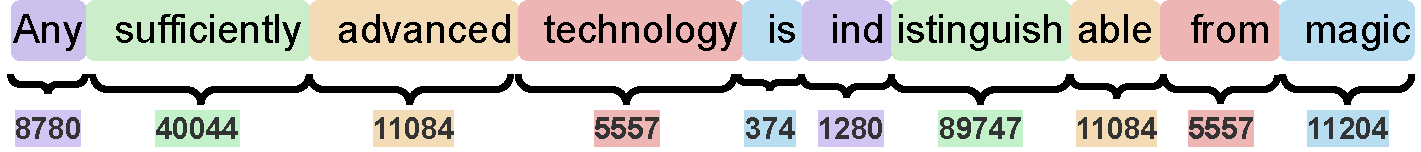
\includegraphics[width=0.98\textwidth]{img/tokenization.pdf}
    \caption{Example tokenization of a sentence for the LLaMA3 tokenizer \citep{LLamaTokenizerPlayground}}
    \label{fig:tokenization}
\end{figure}
This process begins with tokenization, where input text is divided into smaller units called tokens (see Figure \ref{fig:tokenization}).
% These tokens are then converted into numerical vectors (embeddings) that capture semantic meaning. Following that, they then get processed in the core of the transformer model: Multiple layers of self-attention and feed-forward neural networks. In self-attention layers, the model learns to identify relevant relationships between all tokens in the sequence. Subsequently, feed-forward layers further process this information and contain most of the models knowledge. The model then decodes this processed information to generate output text. Decoding happens token by token, with each new token being influenced by all previous tokens, until an end-of-sequence token is produced. As a result of this iterative process, the model can generate coherent and contextually relevant text.
Tokens are then transformed into numerical vectors (embeddings) that encapsulate semantic meaning. Subsequently, they are processed through the core of the transformer model: multiple layers of self-attention mechanisms and feed-forward neural networks. Within the self-attention layers, the model learns to identify and weigh relevant relationships between all tokens in the sequence. Following this, feed-forward layers further refine this information, effectively storing the model's knowledge. The model then decodes this processed information to generate output text. This decoding runs sequentially, with each new token being influenced by all preceding tokens, until an end-of-sequence token is produced. As a result of this iterative process, the model can generate coherent and contextually relevant text.

LLMs can be categorized into encoder-only (e.g. BERT \citep{Devlin2018}), decoder-only (e.g. GPT, LLaMA etc.. \citep{Brown2020,LLaMA3}) and encoder-decoder models (e.g. T5 \citep{Raffel2019}), each with its own strengths and weaknesses. Currently most advanced models are based on the decoder-only architecture. For a way more thorough explanation of LLMs and overview I recommend the reader to check out \cite{Zhao2023}.

LLMs have shown to be capable of generating coherent and contextually relevant text, making them suitable for a wide range of applications such as text generation, translation and summarization. But they have also some drawbacks and limitations: Due to their large size and complexity, they require significant computational resources during inference and training. Moreover, they are very sensitive to the quality and quantity of the training data, which can lead to bad quality responses or even worse, biased or harmful outputs.

\section{Fine-tuning}
\label{s:background_finetuning}
Fine-tuning is a technique for adapting a model trained on a broad, generalized dataset. It involves further training the model on a smaller, task-specific dataset, leveraging the model's general knowledge. Fine-tuning leads to small adjustments in the model's weights, which allows it to adapt to the specific task or domain resulting in improved performance. To make fine-tuning even more efficient, there are advanced techniques like low rank adaptation - often referred to as LoRa \citep{Hu2021}. It involves adding trainable rank decomposition matrices to the model's existing weights. This approach significantly reduces the number of trainable parameters, making fine-tuning more memory-efficient and faster, while still achieving comparable performance than traditional fine-tuning.

\section{Language Proficiency and CEFR}
\label{s:background_cefr}
Language proficiency describes the ability of an individual to use a language effectively and accurately in a variety of contexts and situations. The Common European Framework of Reference for Languages (CEFR) is a widely used framework that provides a standardized scale for assessing language proficiency. It divides language proficiency into six levels, ranging from A1 (beginner), A2 (elementary), B1 (intermediate), B2 (upper-intermediate), C1 (advanced) and C2 (proficient). The CEFR is used in language education and assessment to evaluate and certify language proficiency, and it provides a common reference point for language learners, teachers and institutions. There are rules and guidelines for each level, which describe the skills that learners should have at each level. For example, at the A1 level, learners should be able to understand and use familiar everyday expressions and basic phrases, while at the C2 level, learners should be able to understand complex texts and communicate fluently and spontaneously in a variety of contexts.
\section{Challenges in Language Proficiency Classification}
\label{s:background_challenges_classification}
Language proficiency classification is a challenging task, especially for traditional NLP techniques, due to the complexity and ambiguity of human language. There are no explicit rules that can be followed by a traditional algorithm to determine the proficiency level of a text, and the classification is often subjective and context-dependent. Moreover, the classification of language proficiency is not a binary decision, but rather a continuous scale, which makes it difficult to define clear boundaries between the different levels. This is further complicated by the fact that language proficiency is not only determined by the vocabulary and grammar used in a text, but also by the context, style and tone. For example, a text that uses simple vocabulary and grammar may still be classified as advanced if it discusses complex topics or uses sophisticated arguments. Traditional approaches to language proficiency classification rely on manual annotation and expert judgment, which are time-consuming and expensive. They also suffer from subjectivity and inconsistency, as different annotators may have different opinions on the proficiency level of a text. Here LLMs can provide a solution as they are designed to work with natural language text and have shown to be capable of understanding and working with the complexity and ambiguity of human language.
\section{Challenges in Text Transformation}
\label{s:background_challenges_transformation}
Text adaptation is the process of modifying a text to make it more suitable for a specific audience or purpose. In the context of language proficiency, text adaptation involves modifying a text to match the proficiency level of the reader. This can include simplifying the vocabulary and grammar, rephrasing complex sentences  and adding explanations or examples to make the text more understandable. Transferring is an even more challenging task than language proficiency classification, as it requires not only an understanding of the text itself, but also the ability to generate new text that is coherent and contextually relevant while matching the target proficiency level. Problems like this fit LLMs capabilities even more as they are designed to generate text and have shown to be capable of adapting text to different styles and contexts. Transformers are particularly well-suited for this task, as they were originally designed for translation between languages \citep{Vaswani2017} and translation of proficiency levels can be seen as a subset of that task.
\section{Existing Solutions and their Limitations}
\label{s:background_existing_solutions}
There are some approaches to CEFR classification of German texts. Notably there is the work of \cite{Szuuegyi2019}, \cite{Vajjala2018} and extending on that work, \cite{Caines2020}. These approaches all use traditional NLP techniques and machine learning algorithms to classify German (and other languages) texts according to the CEFR levels. They rely on linguistic features such as vocabulary, grammar and syntax to determine the proficiency level of a text. While these approaches have shown promising results, they have some limitations. They are often based on hand-crafted features and rules, which are time-consuming and expensive to create and maintain. Additionally due to their architecture and approach, these methods can not be used to adapt texts to different proficiency levels which is an integral part of this thesis.

\chapter{Methods}
\label{ch:methods}
This chapter outlines the methodology used to evaluate the performance of LLMs in classifying and transferring German texts by CEFR levels. It includes the dataset creation, benchmark design, model selection, data preparation and the fine-tuning process.

\section{Classification Dataset}
\label{s:dataset}
An integral part of any machine learning project is the dataset. Creating a dataset with German CEFR levels was challenging because there are no publicly available datasets with this information for all levels. I had to create a dataset from scratch, combining several existing datasets and using synthetic data generation to create a (balanced) dataset. It consists of about 1,500 texts, each ranging from 500 to 3,000 words. The texts are from different domains, such as simple texts, essays, summaries and more. There are all 6 CEFR levels in the dataset, ranging from A1 to C2. Additional preprocessing steps were taken to ensure the quality of the dataset, such as removing duplicates, removing non-valid characters and more.

\subsection{Creation of the Classification Dataset}
\label{ss:dataset_creation}
The classification dataset was created by integrating multiple existing datasets along with synthetic data generation to ensure a balanced composition. The FALKO Corpus \citep{reznicek2010falko} and MERLIN Corpus \citep{boyd2014merlin} used in this thesis are available under CC BY 3.0 and CC BY-SA 4.0 licenses respectively.
\subsubsection*{Falko Corpus}
\label{sss:falko_corpus}
A significant source utilized was the Falko corpus \citep{reznicek2010falko} collected and annotated at the Humbolt University Berlin. The corpus was designed to facilitate research in corpus linguistics by providing a collection of texts authored by both advanced foreign learners of German and native speakers, collected under controlled conditions and annotated for various linguistic features. From this corpus, the EssayL2, SummaryL1 and SummaryL2 subcorpora were selected due to them containing the necessary data. \\ \\
The \textbf{EssayL2} subcorpora consists of argumentative essays written by foreign learners of German with a CEFR level between B2 and C2. Topics include feminism, financial discussions and crime. All essays of the subcorpora were written under controlled conditions, with the learners having 90 minutes to write each essay. Each essay was then annotated with several metadata points such as the author's age, gender etc... Relevant to me was only the C-test score, which is an integer ranging from 0 to 100 to measure the author's German proficiency. The Falko authors gave a mapping to assign each C-test score to a CEFR level which I used to assign the CEFR level to each essay - see Table \ref{tab:ctest_mapping}.

\begin{table}[ht]
    \centering
    \begin{tabular}{
        >{\raggedright\arraybackslash}p{3cm}
        >{\raggedright\arraybackslash}p{3cm}
        }
        \toprule
        \textbf{Score Range} & \textbf{CEFR Level} \\
        \midrule
        60 - 79 & B2 \\
        80 - 89 & C1 \\
        90 - 100 & C2 \\
        \bottomrule
    \end{tabular}
    \caption{Mapping of C-Test Scores to CEFR Levels}
    \label{tab:ctest_mapping}
\end{table}

The \textbf{SummaryL1} and \textbf{SummaryL2} subcorporas consist of summaries of academic texts written by native speakers of German. The conditions were very similar to the EssayL2 subcorpora, with the learners having 90 minutes to write each summary. While the \textbf{SummaryL1} subcorpus contains summaries written by native speakers and thus processed as C2 samples for my dataset, the \textbf{SummaryL2} subcorpus includes summaries written by learners of German as a second language. \\

This dataset source was rather important as it contains a lot of native speaker texts, which are crucial for the model to understand the C2 level.

\subsubsection*{MERLIN Corpus}
\label{sss:merlin_corpus}
The second primary textual source was the MERLIN corpus \citep{boyd2014merlin}, a learner corpus designed to illustrate the CEFR with authentic learner data. It includes texts in three languages: Italian, Czech and German. There are entries covering all 6 CEFR levels with a strong focus on A2,B1 and B2 levels. Offering a diverse range of text types, including essays, summaries and other forms, the corpus is perfect for this thesis. These texts were collected as part of a standardized language test, which ensures the texts have great consistency and quality. All samples were annotated with CEFR levels by language experts, which guarantees the quality and accuracy of the labels. Due to that I could directly use the CEFR labeled texts provided by the corpus for my dataset.

\subsubsection*{Synthetic Data Generation}
\label{sss:synthetic_data_generation}
To address the scarcity of A1-level texts in the available sources, a synthetic data generation method was employed to enable having a dataset to evaluate across all CEFR levels.
I chose to use the Claude 3.5 Sonnet model \citep{claude3.5sonnet}, an advanced LLM developed by Anthropic due to its versatility in generating high-quality texts, large knowledge base and good prompt adherence \citep{Huang2024}.
The prompt engineering process consisted of several iterations to achieve the desired sample output. Initial attempts resulted in texts that showed a very high similarity to early primary school texts, which was not the desired outcome as I wanted texts in diverse topics to avoid dataset bias. Models would have associated the levels with the topics rather than the complexity of the text samples. To counteract these issues, I adjusted the prompt to avoid typical topics that the model would fall back to. Additionally the model was supplied a definition of the A1 level by the Goethe Institute to guide the model and prevent it from generating texts with higher complexity \citep{goetheCefr}. Also I settled on German as the language for the prompt as it showed better results than an English prompt. \\ \\
The final prompt used for the synthetic data generation was:
\captionsetup{labelformat=prompt}
\begin{figure}[h]
    \begin{quotation}
        \textit{Bitte generiere Texte mit dem CEFR Niveau A1. Diese sollten länger (Circa 600 Wörter) sein. Versuche Themen zu finden, welche nicht mit Schule/Kindheit in Verbindung stehen. Es sollte sich um Texte für Deutsch Sprachler mit dem Level A1 handeln. \\
        Hier ist eine Definition des A1 Levels: \\
        Kann vertraute, alltägliche Ausdrücke und ganz einfache Sätze verstehen und verwenden, die auf die Befriedigung konkreter Bedürfnisse zielen.
        Kann sich und andere vorstellen und anderen Leuten Fragen zu ihrer Person stellen – z. B. wo sie wohnen, welche Leute sie kennen oder welche Dinge sie haben – und kann auf Fragen dieser Art Antwort geben.
        Kann sich auf einfache Art verständigen, wenn die Gesprächspartner langsam und deutlich sprechen und bereit sind zu helfen.}
    \end{quotation}
    \caption{Final German Prompt for Synthetic Data Generation using definition by \cite{goetheCefr}}
    \label{qu:synthetic_prompt}
\end{figure}
\captionsetup{labelformat=default}

Using this I generated a total of 122 texts, which each undergoing a manual review to ensure  quality and relevance before being included in the dataset. \\ \\
While synthetic data generation proved effective for the A1 level, it was deemed unsuitable for the higher CEFR levels due to the complexity of the levels and the model's inability to reliably generate texts of that complexity. I am going to address this problem in the second part of my thesis (Section \ref{s:llm_fine_tuning}). There is also a risk of dataset bias, as the model could have generated texts with a schema that is not directly recognizable by humans. Regardless, this should not pose a problem in this case as the MERLIN dataset also provides A1 samples which were also used and thus the synthetic data is only a part of the dataset, not the whole dataset.

A detailed analysis of the dataset composition, distribution and word count across different CEFR levels is provided in the results chapter in Section \ref{s:classification_dataset_analysis}.

The transformation dataset for the transfer task is addressed later, as it relies on the fine-tuned classification model introduced in the following subsections. For details see Subsection \ref{ss:dataset_generation}.

\begin{table}[ht]
    \centering
    \begin{tabular}{
        >{\raggedright\arraybackslash}p{4cm}
        >{\raggedright\arraybackslash}p{1.25cm}
        >{\raggedright\arraybackslash}p{1.25cm}
        >{\raggedright\arraybackslash}p{1.25cm}
        >{\raggedright\arraybackslash}p{1.25cm}
        >{\raggedright\arraybackslash}p{1.25cm}
        >{\raggedright\arraybackslash}p{1.25cm}
        }
        \toprule
        \textbf{Source} & \textbf{A1} & \textbf{A2} & \textbf{B1} & \textbf{B2} & \textbf{C1} & \textbf{C2} \\
        \midrule
        Falko EssayL2     &     &     & & 83  & 84  & 81    \\ \midrule
        Falko SummaryL1   &     &     &     &  &    & 58   \\ \midrule
        Falko SummaryL2 & & & & & 53 & 53 \\ \midrule
        MERLIN            & 57  & 306 & 331 & 293 & 42 & 4  \\ \midrule
        Synthetic         & 122 &     &     &     &    &    \\ \midrule
        \textbf{Sum (1,567)}      & \textbf{179} & \textbf{306} & \textbf{331} & \textbf{376} & \textbf{179} & \textbf{196} \\
        \bottomrule
    \end{tabular}
    \caption{Data Distribution Across Different Levels}
    \label{tab:data_distribution}
\end{table}
\clearpage

\section{Evaluation Framework and Benchmark Design}
\label{s:evaluation_framework}
\subsection{Definition of Evaluation Metrics}
\label{ss:evaluation_metrics}
\subsubsection*{Classification Task}
\label{sss:classification_task}
Defining the evaluation metrics for the classification task is an important step to ensure the ability to judge the performance of the model and compare it to other models. This allows us to objectively measure the performance increase and the effectiveness of the prompts.
As this task is a very simple classification task (only 6 possible classes), I can use the standard evaluation metrics for classification tasks, consisting of accuracy, precision, recall and F1 score. See Table \ref{tab:common_evaluation_metrics} for a detailed explanation of the metrics.

\begin{table}[ht]
    \centering
    \begin{tabular}{
        >{\raggedright\arraybackslash}p{2cm}
        >{\raggedright\arraybackslash}p{6cm}
        >{\centering\arraybackslash}p{5cm}
        }
        \toprule
        \textbf{Metric} & \textbf{Description} & \textbf{Formula} \\
        \midrule
        Accuracy & Ratio of correctly classified samples to the total number of samples. Provides an overall measure of the model's performance across all classes. Can be misleading in cases of imbalanced datasets. & $\frac{\text{Number of Correctly Classified Samples}}{\text{Total Number of Samples}}$ \\
        \midrule
        Precision & Specific to each class. Ratio of correctly classified samples to the total number of samples classified as that class. Measures the model's ability not to label a sample as a certain class when it is not. & $\frac{\text{True Positives}}{\text{True Positives} + \text{False Positives}}$ \\
        \midrule
        Recall & Specific to each class. Ratio of correctly classified samples to the total number of samples that are actually in that class. Measures the model's ability to find all the samples that belong to a certain class. & $\frac{\text{True Positives}}{\text{True Positives} + \text{False Negatives}}$ \\
        \midrule
        F1 Score & Balances precision and recall, allowing comparison of models based on a single value. & $2 \cdot \frac{\text{Precision} \cdot \text{Recall}}{\text{Precision} + \text{Recall}}$ \\
        \bottomrule
    \end{tabular}
    \caption{Common Evaluation Metrics for Classification Tasks}
    \label{tab:common_evaluation_metrics}
\end{table}

Additionally to these standard metrics, I also introduced another metric called \textit{group accuracy}. As CEFR classifications are inherently subjective due to their language origin \citep{Siddhant2020} and the boundaries between levels are not always clear, it is possible, that different experts classify the same text differently. Therefore there could be a situation where a text is classified as B1 but also as B2 - both classifications could be correct. To account for this, I introduced the group accuracy metric. I define a group as a set of two adjacent CEFR levels. For example, a group consists of A1 and A2, another group of A2 and B1 and so on. The group accuracy is then defined as the ratio of samples that were classified in the correct group to the total number of samples - allowing to measure the model's ability to classify texts in the correct group, even if the exact level is not correct.

\subsubsection*{Transfer Task}
\label{sss:transfer_task}
For the transfer task, the evaluation metrics are substantially more complex. The model is evaluated on its ability to transfer knowledge from one CEFR level to another while retaining the content. Evaluation metrics for this task are two fold:
To begin with, the transferred text undergoes classification to determine if it matches the target CEFR level utilizing the classification LLM. By using the classifier, I ensure a consistent and reliable metric for evaluation. Additionally I determine the group transfer accuracy, similar to the classification task.
% The transferred text's CEFR level is determined using the previously developed classification model. This approach provides a consistent and reliable metric for evaluating the transfer process's accuracy in achieving the target CEFR level.
Secondly, the content retention is evaluated by employing a second (foundation) LLM as a judge model. The LLM is given the original and transferred text while being tasked to evaluate the content similarity between the two texts.
% Only if the target CEFR level is reached and the content is retained, the transfer is considered successful.

\begin{table}[ht]
    \centering
    \begin{tabular}{
        >{\raggedright\arraybackslash}p{2cm}
        >{\raggedright\arraybackslash}p{7cm}
        >{\centering\arraybackslash}p{4cm}
        }
        \toprule
        \textbf{Metric} & \textbf{Description} & \textbf{Methodology} \\
        \midrule
        Transfer accuracy & Ratio of samples where the transferred text is classified as the target CEFR level to the total number of samples. & Classification LLM \\
        \midrule
        Group Transfer accuracy & Ratio of samples where the transferred text is classified as the target CEFR level or the adjacent CEFR level to the total number of samples. & Classification LLM \\
        \midrule
        Content Preservation Rate & Ratio of samples where the content similarity between the original and the transferred text is sufficiently retained, as evaluated by a LLM, to the total number of samples. & Judge LLM \\  \bottomrule
    \end{tabular}
    \caption{Evaluation Metrics for Transfer Tasks}
    \label{tab:evaluation_metrics}
\end{table}

\subsection{Classification Task Benchmark Design}
\label{ss:benchmark_design}
The benchmark for the classification task is designed to evaluate the performance of the classification LLM. In the following, I will define a run as a single evaluation cycle of the model. For each run, a given amount of samples for each CEFR level are selected. Then, using a base model with prompting, the samples are randomly selected from the dataset. If a fine-tuned model is being benchmarked, the samples are selected from the validation split of the dataset for that specific model.

For each sample, the model is tasked to classify the text. The system prompt is set to an instruction and the sample is supplied to the model as the first user message. The model then generates the second message, which is the classification of the text with a limit of 2 tokens.
After the model has generated all predictions, the evaluation metrics are calculated for the whole run (accuracy and group accuracy) and each CEFR level (precision, recall and F1). This process can be repeated multiple times to get a more accurate representation of the model's performance, as with a temperature > 0 the model will generate different outputs for the same input. Final evaluation metrics are then calculated as the average over all runs. For this thesis, I decided on a temperature of 0 for the classification task as this guarantees consistent results. Additionally, testing showed the models seems to perform better with a temperature of 0. This makes sense due to the model only having to generate two tokens, which would be massively skewed by a higher temperature. Additionally this choice also provides reproducibility, as the results are consistent across runs.

Accompanying the benchmark, I developed a small web interface to allow for easy testing of the model. The interface allows the user to select a model and benchmark parameters such as the number of runs, temperature, sample size, system prompt and more. It then automatically runs the benchmark and displays the runs in an easy to read list. For each run the user can access a detailed view, showing the run results in a confusion matrix and the evaluation metrics for each CEFR level. This allows for easy and fast comparison of different models and benchmark parameters. Additionally, the interface has some additional features such as the ability to abort runs that result in a lot of miss-classifications in direct succession, indication an issue with the model or prompt. \\


\section{CEFR Classification via Prompt Engineering}
\label{s:prompt_engineering}
\subsection{Prompt Design Strategy}
\label{ss:prompt_design}
I started the prompt design process by choosing a first base model to start working with to evaluate my prompts. This choice turned out to be the LLaMA3-8B model \citep{LLaMA3} as it is rather small and thus has fast inference times, allowing for quick testing of prompts. Later on I chose the best performing model, see Subsection \ref{ss:base_model_selection}. The prompt design process was iterative and consisted of several steps, each improving on the previous one. With the end goal being to design a prompt that instructs the model to effectively classify the CEFR level of a given text.

\subsubsection*{Basic Prompt}
\label{sss:basic_prompt}
Initial steps involved designing a simple prompt instructing the model to classify the first text supplied by the user in the conversation. Two parts are integral to the prompt: First a simple description of the model's task and secondly a list of valid responses for the model to chose from. I decided first try to design the prompt in English, as the model was mostly trained on English data \citep{LLaMA3} and that should lead to better instruction adherence. Similar behavior is common in LLMs as shown by \cite{Siddhant2020}. The performance of this prompt was evaluated, with results available in the appendix \ref{tab:first_english_prompt}.
\captionsetup{labelformat=prompt}
\begin{figure}[h]
    \begin{quotation}
        \textit{Classify the language level of a given text according to the Common European Framework of Reference for Languages (CEFR). Respond with only the corresponding CEFR level (A1, A2, B1, B2, C1 or C2).}
    \end{quotation}
    \caption{First English Prompt}
    \label{qu:first_english_prompt}
\end{figure}
\captionsetup{labelformat=default}

\subsubsection*{German Zero-Shot Prompt}
\label{ss:german_zero_shot_prompt}
The evaluation of the previous prompt showed some problems. To address these shortcomings, a switch to German was made, based on two considerations:
\begin{enumerate}
    \item First, as the classification task is designed for German texts, using a German prompt could potentially profit from more relevant language knowledge in the model. Also as German has the same origin as English, the languages share some similarities. \cite{Pires2019} has shown, that LLMs can better adapt to languages, that are similar to the ones they were mostly trained on. So this could potentially lead to better results.
    \item Secondly, the model had already shown good adherence to instructions, suggesting that the problem remains in the classification task itself rather than in understanding and following the prompt.
\end{enumerate}
The new prompt is a direct translation of the English prompt, with minor adjustments to ensure natural phrasing in German and a focus on the valid responses.
\captionsetup{labelformat=prompt}
\begin{figure}[h]
    \begin{quotation}
        \textit{Bewerte die Sprachkenntnisse des bereitgestellten deutschen Textes gemäß dem Gemeinsamen Europäischen Referenzrahmen für Sprachen (GER/CEFR). Antworte NUR mit der entsprechenden Stufe: A1, A2, B1, B2, C1 oder C2, *keiner* Begründung}
    \end{quotation}
    \caption{German Zero-Shot Prompt}
    \label{qu:german_prompt}
\end{figure}
\captionsetup{labelformat=default}

The effectiveness of this German prompt was assessed through comparative testing against its English counterpart showing slight improvement in the model's performance. See the appendix Table \ref{tab:zero_shot_confusion_matrix} for the results.

% This lead to a small improvement in the model's performance, with the overall accuracy increasing to 33.3\% and the group accuracy rising to 75.3\%. The model started to show substantial improvements in classifying A1-A2 and C1-C2 levels. However there still was a rather string bias towards the B1 and B2 levels, albeit less pronounced than with the English prompt. This persistent bias might be attributed to these intermediate levels representing a "middle ground" in language proficiency, making them harder to distinguish from adjacent levels.
% While the German prompt showed promise, the accuracy levels were still not good enough. This led to the exploration of more advanced prompting techniques, as discussed in the following section.

\subsubsection*{German Few-Shot Prompt}
\label{ss:few_shot_prompt}
For now all prompts were zero-shot prompts, meaning that the model was not given any examples with desired output beforehand. To further increase performance, a few-shot prompt was designed, where the model is given a few text samples with their corresponding CEFR level. 
As shown by \cite{Brown2020}, this should help the model to better understand the task and improve its performance. The few-shot prompt can be seen in Prompt \ref{qu:few_shot_prompt}.

\captionsetup{labelformat=prompt}
\begin{figure}[h]
    \begin{quotation}
        \textit{Klassifiziere die Sprachkenntnisse des bereitgestellten deutschen Textes gemäß dem Gemeinsamen Europäischen Referenzrahmen für Sprachen (GER/CEFR). Antworte NUR mit der entsprechenden Stufe: A1, A2, B1, B2, C1 oder C2, NICHT MEHR. Gebe auch *keine* Begründung! \\
        Hier sind jeweils Beispiele: \\ \\
        A1: Lieber Jens, Ich Glückwünsche dich ist Vater geworden. Wie es deine Frau und deine Babys? Wie heißt des Babys? Brauchst du etwas hilfe? Könntest du bitte mich anrufen? Herzlichen Grüßen Maria Meier \\
        A2: [...] \\
        B1: [...] \\
        B2: [...] \\
        C1: [...] \\
        C2: [...]}
    \end{quotation}
    \caption{German Few-Shot Prompt, shortened (See Prompt \ref{qu:few_shot_prompt_complete} for full version)}
    \label{qu:few_shot_prompt}
\end{figure}
\captionsetup{labelformat=default}

For readability reasons I only included the A1 example in the prompt, the other examples are similar in structure and content. Also note that the grammar and spelling mistakes are intentional, as they are typical for the respective CEFR level and the sample was taken from a real text. See the appendix at Prompt \ref{qu:few_shot_prompt_complete} for the full version.

This prompt incorporates an example with its corresponding class for each CEFR level. All examples were specifically selected from samples that the model had previously misclassified, with the aim of enhancing the model's understanding of the task and improving its performance. \\
% TODO: move to results
% The few-shot prompt showed a significant improvement in the model's accuracy, which increased to 59.3\%, while the group accuracy rose to 94.0\%. Additionally, the bias towards the B1 and B2 levels was also reduced. However, the model still showed difficulties with classifying texts at the A2 and C1 levels, as shown in Table \ref{tab:few_shot_confusion_matrix}. These persistent problems with A2 and C1 classifications may stem from them being between the two endpoints and middle levels. While it is relatively easy to distinguish between very simple, medium, and highly complex texts (corresponding to A1, B1/B2, and C2 levels respectively), the differences in the middle levels are harder to distinguish.
Additional experimentation with prompting did not yield any further improvements in accuracy. Notably, the inclusion of additional examples in the prompt did not result in significant improvements - in fact, it led to a slight decrease in classification accuracy. This effect may be caused by potential overfitting, where the model becomes too closely aligned with the specific examples provided in the prompt, potentially hampering its ability to generalize to new, unseen texts. 

\subsection{Base Model Selection}
\label{ss:base_model_selection}
\subsubsection*{Selection Criteria}
\label{sss:selection_criteria}
After refining the prompt with a stand-in model I decided to evaluate different models to find the best one. Before deciding on a model, I first had to define the selection criteria. \\
The most important criterion was the model's performance on the classification task, mainly the accuracy and group accuracy scores.
Additionally the model's parameter count and inference time were also considered for two reasons. Firstly, a small(er) model (<30B parameters) would allow for faster inference times, thus being more effective and practical for real world use. Secondly, a smaller model would also be easier to fine-tune, as it requires less computational resources.  \\
% This is not as important for the classification task, but becomes crucial for the transfer task, where a fine-tuning step is likely to be performed. \\
Lastly, the model's adherence to the prompt was also considered. For the classification task the model needs to only respond with the CEFR level, nothing else. If the models does not adhere to the prompt and provides additional information or argumentation, it is considered a wrong classification and results in worse performance. \\
Also important was, that the model has open weights and can be fine-tuned. This criteria includes the right license for research fine-tuning.

\subsubsection*{Possible Models}
\label{sss:possible_models}
The following models were considered for evaluation:
% \begin{itemize}
%     \item Meta-LLaMA-3-8B-Instruct \cite{LLaMA3}
%     \item Meta-LLaMA-3-70B-Instruct \cite{LLaMA3}
%     \item Mistral-7B-Instruct \cite{Jiang2023}
%     \item Mixtral-8x22B-Instruct-v0.1 \cite{Jiang2023}
%     \item google/gemma-2-9b-it \cite{GemmaTeam2024}
%     \item google/gemma-2-27b-it \cite{GemmaTeam2024}
%     \item qwen/qwen2-7B-Instruct \cite{Yang2024}
%     \item qwen/qwen2-72B-Instruct \cite{Yang2024}
% \end{itemize}
\begin{table}[ht]
    \centering
    \begin{tabular}{
        >{\raggedright\arraybackslash}p{5cm}
        >{\arraybackslash}p{4.5cm}
        }
        \toprule
        \textbf{Model Name} & \textbf{Reference} \\
        \midrule
        Meta-LLaMA-3-8B-Instruct & \cite{LLaMA3} \\
        \midrule
        Meta-LLaMA-3-70B-Instruct & \cite{LLaMA3} \\
        \midrule
        Mistral-7B-Instruct & \cite{Jiang2023} \\
        \midrule
        Mixtral-8x22B-Instruct-v0.1 & \cite{Jiang2023} \\
        \midrule
        google/gemma-2-9b-it & \cite{GemmaTeam2024} \\
        \midrule
        google/gemma-2-27b-it & \cite{GemmaTeam2024} \\
        \midrule
        qwen/qwen2-7B-Instruct & \cite{Yang2024} \\
        \midrule
        qwen/qwen2-72B-Instruct & \cite{Yang2024} \\
        \bottomrule
    \end{tabular}
    \caption{Language Models Considered for Evaluation}
    \label{tab:llm_models}
\end{table}

% \subsubsection*{Selected Model}
% \label{sss:selected_model}
% After evaluating all models based on their performance, size and license, I determined the Meta-LLaMA-3-8B-Instruct model to be the best choice for the classification task and further fine-tuning. For further results see the appendix \ref{tab:base_model_selection}.

\subsubsection*{Selected Model}
\label{sss:selected_model}
After evaluating all models based on their performance, size and license, I determined the Meta-LLaMA-3-8B-Instruct model to be the best choice for the classification task and further fine-tuning. The selection process considered several key factors:

\begin{enumerate}
    \item Performance: The model's accuracy and group accuracy were evaluated on a subset of the dataset. While specific results are presented in the Results section at \ref{fig:llm-performance-comparison}, the LLaMA-3-8B-Instruct model demonstrated competitive performance.
    \item Model Size: With 8 billion parameters, this model offers a good balance between capability and computational efficiency. This was an important consideration for both fast inference speed and the ability to fine-tune the model effectively and iterate quickly.
    \item Open Weights: The availability of open weights was crucial for this thesis, as it allows for fine-tuning and adaptation to the specific tasks.
    \item Licensing: The model's license permits research use and fine-tuning, which aligns with this thesis needs.
    \item Architecture: The LLaMA-3-8B-Instruct model uses a transformer architecture optimized for instruction following, which is well-suited for the classification and transfer tasks.
\end{enumerate}

While larger models were available, the LLaMA-3-8B-Instruct model offered the best compromise between performance and resource requirements. The detailed performance comparisons that led to this selection, including accuracy and group accuracy metrics for all evaluated models can be found in the appendix at \ref{fig:llm-performance-comparison}.

It is important to mention, that the model selection process has a slight bias towards the LLaMA-3-8B-Instruct model. As the evaluation of the different models was done on the manually refined prompt, which was designed with the LLaMA-3-8B-Instruct model as a stand-in. This could potentially lead to a bias towards this model, as the prompt was iteratively designed to work well with this model. It could be, that with other prompts the results would be different and another model would be better contenders. As the prompt showed good results with several other models as well, the bias should be minimal but still needs to be mentioned and kept in mind.
\section{CEFR Classification via LLM Fine-Tuning}
\label{s:llm_fine_tuning}

After exploring prompting for the classification task, I moved on to fine-tuning a model on the classification task to see if this would lead to better results. Fine-tuning involves further training of an already pre-trained model on a dataset to adapt the model to a specific task or domain. This will allow the model to learn patterns and features relevant to the CEFR classification task. In this section I will discuss dataset preparation and the process of fine-tuning itself.

\subsubsection{Model Selection}
\label{sss:model_selection}
Based on Subsection \ref{ss:base_model_selection} I decided to fine-tune the Meta-LLaMA-3-8B-Instruct model. This model showed the best performance on the classification task and adhered well to the prompt. Additionally, the model has a relatively small parameter count, which should allow for faster fine-tuning and inference times. LLaMA3 also has open weights and is licensed for research fine-tuning \citep{LLaMA3}.

\subsubsection{Dataset Preparation}
\label{sss:dataset_preparation}
To prepare the dataset I first randomly selected 179 samples from each CEFR level. This was done do avoid any bias towards the center levels as these were overrepresented in the dataset (See Table \ref{tab:data_distribution}) and 179 samples is the lowest number of samples for a CEFR level. The samples were then split into two parts:
\begin{itemize}
    \item Training data: 154 per CEFR level to be used for fine-tuning the model
    \item Test data: 25 samples per CEFR level to be used for evaluation of the fine-tuned model
\end{itemize}
All texts were formatted for the fine-tuning process. Each sample was formatted as a single string that conforms to the LLAMA 3 input format, consisting of a system prompt, a user message and the assistant response separated by special tokens. 
Special tokens are tokens that are not part of the normal text embedding vocabulary and used to separate the different parts of the input and indicate end of the models response. A shortened version of the prompt used for the classification task was used as the system prompt, removing the examples for each CEFR level as they will be implicitly learned by the model during fine-tuning. The first user message was set to the sample to be classified by the model. Then the assistant response was set to the correct CEFR level. See Prompt \ref{qu:formatted_sample} for an example of a formatted sample.

\captionsetup{labelformat=prompt}
\begin{figure}
    \begin{quotation}
        \textcolor{gray}{<|start\_header\_id|>}\textcolor{blue}{system}\textcolor{gray}{<|end\_header\_id|>}Klassifiziere das Sprachniveau des bereitgestellten deutschen Textes gemäß dem Gemeinsamen Europäischen Referenzrahmen für Sprachen (GER/CEFR). Antworte NUR mit der entsprechenden Stufe: A1, A2, B1, B2, C1 oder C2, NICHT MEHR.\textcolor{gray}{<|eot\_id|>}\textcolor{gray}{<|start\_header\_id|>}\textcolor{blue}{user}\textcolor{gray}{<|end\_header\_id|>}\textcolor{orange}{[SAMPLE]}
        \textcolor{gray}{<|eot\_id|>}\textcolor{gray}{<|start\_header\_id|>}\textcolor{blue}{assistant}\textcolor{gray}{<|end\_header\_id|>}\textcolor{orange}{[CORRECT SAMPLE CLASS]}\textcolor{gray}{<|eot|>}
    \end{quotation}
    \caption{Formatted Prompt Sample for Fine-Tuning}
    \label{qu:formatted_sample}
\end{figure}
\captionsetup{labelformat=default}

Then all formatted samples were scrambled to avoid any problems in the training process due to class repetition.

\subsubsection{Fine-Tuning Process}
\label{sss:fine_tuning_process}
The fine-tuning process was conducted using Unsloth, which is specifically designed for efficient fine-tuning of LLMs. Training was carried out on an NVIDIA GPU, leveraging PyTorch for the underlying computations.
I used llama-3-8b-Instruct as the base model, with a maximum sequence length of 4096 tokens. The model was loaded in 16-bit precision (float16) to achieve best computational accuracy. To ensure efficient resource usage for the fine-tune I employed Low-rank Adaptation with a rank of 64 and a dropout of 0.

The following hyper-parameters were used for the fine-tuning itself:

\begin{table}[ht]
    \centering
    \begin{tabular}{ll}
        \toprule
        \textbf{Hyperparameter} & \textbf{Value} \\
        \midrule
        Learning rate & 2e-4 \\
        Number of epochs & 5 \\
        Batch size & 1 \\
        Gradient accumulation steps & 1 \\
        Warmup steps & 400 \\
        Weight decay & 0.001 \\
        Learning rate scheduler & Linear \\
        \bottomrule
    \end{tabular}
    \caption{Hyperparameter Used for Fine-tuning}
    \label{tab:fine_tuning_hyperparameters}
\end{table}
The learning rate of 2e-4 was chosen as it is recommended by the Unsloth authors as a good starting point for fine-tuning LLMs, balancing between learning speed and stability \citep{unsloth2024}. I ran the training for 5 epochs, which was determined to be sufficient for the model to converge on the task without overfitting, based on previous experiments. These showed that the loss was not decreasing significantly after the 5th epoch. Additionally, there was no increase in performance for these runs. I chose a batch size of 1 as I wasn't constrained by memory with the 8B parameters of the model. For the optimizer I chose the AdamW optimizer in the 8-bit variant. AdamW is an extension of the Adam optimizer that implements decoupled weight decay regularization, which can help with reducing overfitting \citep{Loshchilov2017}. I chose not to implement any additional overfitting protection, as previous experiments showed no real danger of that occurring with the 5 epochs chosen for this fine-tuning approach.

The fine-tuning was performed on an NVIDIA RTX A6000 GPU. This GPU has 48GB of VRAM, which was sufficient for fine-tuning the 8B parameter model. The process was implemented using PyTorch \citep{Paszke2019} as the underlying framework, with Unsloth providing optimizations specific to LLM fine-tuning. Fine-tuning took approximately 20 minutes to complete the 5 epochs. During training the loss and learning rate were monitored to avoid overfitting and ensure an efficient training.

In the end the LoRa adapter was merged with the base model to create the final fine-tuned model with 16bit precision. This model was then evaluated on the test data to determine its performance on the classification task. Results of this evaluation are presented in the results section at \ref{sss:best_finetuning_evaluation}.

\section{Text Adaptation through LLM Fine-Tuning}
\label{s:llm_fine_tuning}
\subsection{Dataset Generation}
\label{ss:dataset_generation}
The existing dataset created in Subsection \ref{sss:dataset_preparation} contained only the original text samples and their corresponding CEFR levels. To do the transfer task fine-tuning I needed to create a new dataset that contained the text samples in multiple CEFR levels. As it was not practical to manually create such a dataset, I decided to use synthetic data generation. In the initial dataset generation step, this was not possible due to the inability to correctly classify generated data. Despite this, with the fine-tuned model from \ref{sss:fine_tuning_process}, I was able to use a different approach. \\

\begin{figure}[h]
    \centering
    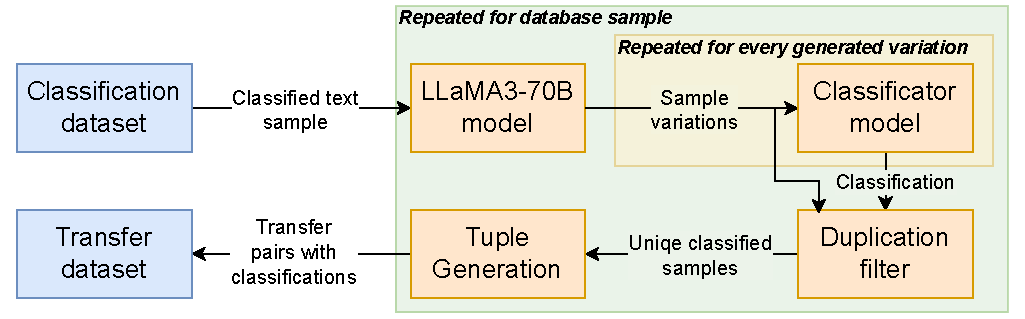
\includegraphics[width=\textwidth]{img/TransferDatasetCreation2.pdf}
    \caption{Dataset Generation Process for Text Adaptation}
    \label{fig:dataset_generation_process}
\end{figure}

\subsubsection*{Dataset Generation Process}
\label{sss:dataset_generation_process}
I ended up using another foundation model to generate the synthetic data and verify the correct classification using the fine-tuned model.
The generation process began by iterating trough all samples in the original dataset to serve as a "base" sample for adaptation. For every base text, I instructed a base LLaMA3-70B model (See Prompt \ref{qu:adaptation_prompt}) to generate adapted versions of the base sample in all CEFR levels while preserving the original content and meaning. This approach was designed to maintain consistency in the content across different proficiency levels. The model was specifically directed to produce all versions at once, a strategy that allowed it to consider the context of lower-level transformations while generating higher-level versions. Ensuring a coherent progression in language complexity across the CEFR levels.

\captionsetup{labelformat=prompt}
\begin{figure}[h]
    \begin{quotation}
        \textit{
            Erstelle bitte Varianten des folgenden Textes in allen CEFR Niveaus, außer dem Originalniveau \textcolor{orange}{[ORIGINAL LEVEL]}: \\ \\
            "\textcolor{orange}{[SAMPLE TEXT]}" \\ \\
            Die Texte sollten den gleichen Inhalt haben, aber an das jeweilige CEFR Niveau angepasst sein. Gebe die Texte als JSON Objekt mit CEFR-Leveln als Keys zurück und antworte NUR mit dem Objekt, keine Begründungen, keine Codeblöcke(```), keine Erklärungen dass du etwas nur versuchen kannst oder ähnliches! Und stelle sicher, dass die Texte den gleichen Inhalt haben, sonst wirst du gefeuert!
        }
    \end{quotation}
    \caption{Prompt for Broad Text Adaptation}
    \label{qu:adaptation_prompt}
\end{figure}
\captionsetup{labelformat=default}

After the generation, each newly generated sample underwent classification by the fine-tuned model, ensuring the correct classification of the generated samples the quality of the new dataset. The samples were then filtered to remove multiple transformed samples in the same CEFR level. As a final step, all possible combinations of two-pair samples were generated, including bidirectional transformations. This was done to ensure that the model would be exposed to a diverse range of CEFR level transitions during training.

See Table \ref{tab:transfer_distribution} for an overview of the distribution of the generated samples.

\begin{table}[ht]
    \centering
    \begin{tabular}{
      >{\raggedright\arraybackslash}p{2.5cm}
      >{\raggedright\arraybackslash}p{2cm}
      >{\raggedright\arraybackslash}p{2cm}
    }
        \toprule
        \textbf{Transfer Type} & \textbf{Count} & \textbf{Percentage} \\
        \midrule
        A1 $\leftrightarrow$ C1 & 250 & 20.63\% \\
        A1 $\leftrightarrow$ C2 & 236 & 19.47\% \\
        A2 $\leftrightarrow$ C2 & 174 & 14.36\% \\
        A2 $\leftrightarrow$ C1 & 160 & 13.20\% \\
        A1 $\leftrightarrow$ B2 & 126 & 10.40\% \\
        A1 $\leftrightarrow$ B1 & 66 & 5.45\% \\
        A2 $\leftrightarrow$ B2 & 64 & 5.28\% \\
        B1 $\leftrightarrow$ C1 & 54 & 4.46\% \\
        B1 $\leftrightarrow$ C2 & 46 & 3.80\% \\
        B2 $\leftrightarrow$ C2 & 14 & 1.16\% \\
        A2 $\leftrightarrow$ B1 & 10 & 0.83\% \\
        B2 $\leftrightarrow$ C1 & 8 & 0.66\% \\
        A1 $\leftrightarrow$ A2 & 4 & 0.33\% \\
        \midrule
        \textbf{Total entries} & \textbf{1212} & \textbf{100\%} \\
        \bottomrule
    \end{tabular} \\
    \textit{Note: Bidirectional transformations are combined for better readability. See Table \ref{tab:detailed_transfer_distribution} for a detailed version.} \\
    \caption{Transfer Distribution Overview}
    \label{tab:transfer_distribution}
\end{table}

\phantom{} % Needed as LaTeX breaks without it and some figures disappear into a digital abyss. Idk why, but it works this way.

\subsection{Fine-Tuning Preparation // Dataset Preparation}
\label{ss:fine_tuning_preparation}
After generating the synthetic dataset with multiple CEFR levels for each original sample, I prepared the data for the fine-tuning process. This preparation involved several key steps to ensure the integrity and balance of the training and test sets.

The first step in the preparation process was bidirectional grouping. The dataset contains bidirectional transformations (e.g., A1->C1 and C1->A1) for each pair generated from the original samples. To prevent potential contamination between training and test sets, these bidirectional transformations were grouped together. By doing so, related transformations are treated as a unit throughout the preparation and splitting process.

Following the bidirectional grouping, I used a level pair balancing strategy. The transformations were grouped by CEFR level pairs (e.g., A1->C1, B1->C2). To ensure a balanced representation of all level pairs, I set minimum and maximum limits for the number of samples in each pair. This helps to prevent bias towards certain level transformations and ensures that the model is exposed to a diverse range of CEFR level transitions during training.

With the dataset grouped and balanced, I split it into training and test sets. The split was designed to maintain the integrity of the bidirectional groups by keeping those always together. Approximately 80\% of the samples were allocated to the training set, to be used for fine-tuning the model. Importantly, this set includes at least one sample from each CEFR level pair, ensuring complete coverage during training. The remaining 20\% of the samples were used as the test set.

For the transfer task, I designed a specific user prompt template to instruct the model to adapt the text to a specific CEFR level. The prompt was crafted to be clear, concise and explicit in its instructions to ensure the model's adherence to the task.
% The German language was chosen for the prompt to maintain consistency with the task of transforming German texts.
% The prompt template is shown in Prompt \ref{qu:single_adaptation_prompt}.
\captionsetup{labelformat=prompt}
\begin{figure}[h]
    \begin{quotation}
        \textit{
            Übersetze den folgenden deutschen Text auf das CEFR-Sprachniveau \textcolor{orange}{[TARGET LEVEL]}, während du den ursprünglichen Inhalt und die Bedeutung so weit wie möglich beibehältst: \\ \\
            \textcolor{orange}{[ORIGINAL TEXT]}
        }
    \end{quotation}
    \caption{Prompt for Text Adaptation}
    \label{qu:single_adaptation_prompt}
\end{figure}
\captionsetup{labelformat=default}

% It was designed to clearly specify the target CEFR level, emphasize the importance of maintaining the original content and meaning, and providing a clear structure for the model to follow.

Each sample consisting of an original text, transferred text, original level and target level was then formatted into a format suitable for fine-tuning the LLaMA3 model. The format was the same as in Section \ref{s:llm_fine_tuning} and used the Prompt \ref{qu:single_adaptation_prompt} for the first user message. See Prompt \ref{qu:formatted_adaptation_sample} for an template of a formatted sample.

\subsection{Fine-Tuning Process}
\label{ss:fine_tuning_process}
The fine-tuning was conducted using the same setup as in Section \ref{sss:fine_tuning_process}. Most hyperparameter were kept the same, with the two differences being that the model was only trained for 3 epochs and on a different dataset. This was determined to be sufficient for the model to adapt to the new task without overfitting as the dataset was rather small due insufficient data sources. Completing the fine-tuning process took approximately 10 minutes. The final fine-tuned model was then evaluated on the test data using the metrics defined in \ref{sss:transfer_task}. Results of this evaluation are presented in the results section \ref{sss:best_finetuning_evaluation}.

\captionsetup{labelformat=prompt}
\begin{figure}[h]
    \begin{quotation}
        \textit{
            \textcolor{gray}{<|start\_header\_id|>}\textcolor{blue}{system}\textcolor{gray}{<|end\_header\_id|>}Transformiere den gegebenen deutschen Text auf das angegebene CEFR-Niveau, während du die ursprüngliche Bedeutung beibehältst.\textcolor{gray}{<|eot\_id|>} \\
            \textcolor{gray}{<|start\_header\_id|>}\textcolor{blue}{user}\textcolor{gray}{<|end\_header\_id|>}\textcolor{orange}{[USER PROMPT]}Ziel-CEFR-Niveau: \textcolor{orange}{[TARGET NIVEAU]}\textcolor{gray}{<|eot\_id|>} \\
            \textcolor{gray}{<|start\_header\_id|>}\textcolor{blue}{assistant}\textcolor{gray}{<|end\_header\_id|>}\textcolor{orange}{[TRANSFERRED TEXT]}\textcolor{gray}{<|eot\_id|>}
            }
        \end{quotation}
        \caption{Formatted Prompt Sample for Fine-Tuning}
        \label{qu:formatted_adaptation_sample}
\end{figure}
\captionsetup{labelformat=default}

\subsection{Benchmark Design}
\label{sss:transfer_benchmark}
The transformation benchmark was designed to evaluate the model's ability to adapt German texts between different CEFR levels while maintaining content integrity, utilizing both the fine-tuned transfer model and the classification model.

\begin{figure}[h]
    \centering
    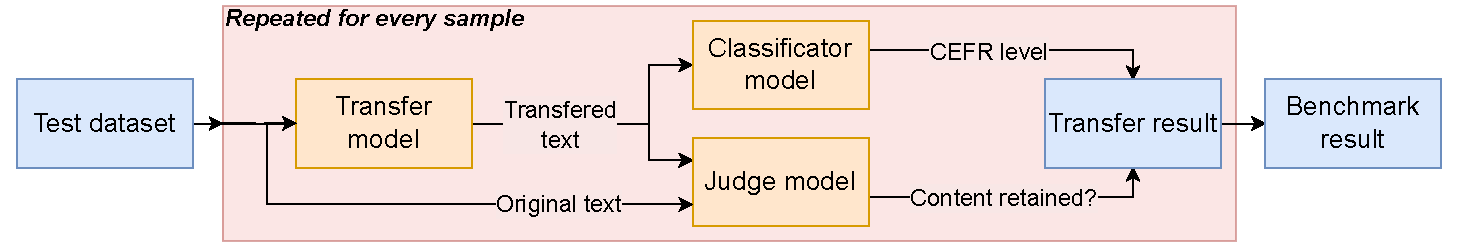
\includegraphics[width=\textwidth]{img/TransferBenchmark3.pdf}
    \caption{Transfer Benchmark Design}
    \label{fig:transfer_benchmark}
\end{figure}

The test dataset consists of samples containing original texts, their CEFR levels and target levels for transformation. For each sample, the original text and target CEFR level are fed into the transfer model using the adapted Prompt \ref{qu:single_adaptation_prompt}.
The model then generates a transformed version of the text, aiming to match the target level. This generated text is then classified using the classification model. To assess content preservation, a separate "judge" model evaluates the similarity between the original and transformed texts. For that I designed Prompt \ref{qu:content_retention_prompt}. I selected LLAMA-3-70B-Instruct \citep{LLaMA3} as the judge model, as it showed promising results in previous experimental testing.

\captionsetup{labelformat=prompt}
\begin{figure}[h]
    \begin{quotation}
        \textit{Original: \textcolor{orange}{[ORIGINAL TEXT]} \\
        Transferred: \textcolor{orange}{[TRANSFERRED TEXT]} \\
        Haben diese beiden Texte das gleiche Thema und selben Inhalt? Antworte nur mit 'Ja' oder 'Nein'.}
    \end{quotation}
    \caption{Content retention prompt}
    \label{qu:content_retention_prompt}
\end{figure}
\captionsetup{labelformat=default}

After all test samples were processed, the evaluation metrics are calculated. This includes the transformations transfer accuracy, group transfer accuracy and content preservation scores. All results of this benchmark are presented and evaluated in the following results Section \ref{s:transfer_results}.

\chapter{Results}
\label{ch:results}
This chapter presents the findings from my research into the use of LLMs for classifying and transferring between German language proficiency levels. The results are organized according to the two main tasks: CEFR classification and proficiency level transfer. I first present the outcomes of the classification tasks using both prompt engineering and fine-tuning approaches. This is then followed by the results of my text transfer experiments. For each set of results, I provide quantitative metrics, visualizations and a brief description of key findings.

\section{Classification Dataset Analysis}
\label{s:classification_dataset_analysis}
\subsection*{Dataset Composition}
\label{ss:dataset_composition}
The classification dataset consists of 1,445 text samples across all six CEFR levels (A1,A2,B1,B2,C1,C2). The distribution of the samples across the different levels is shown in Table \ref{tab:data_distribution}. Notably, the distribution is not uniform across all levels - A2, B1 and B2 have a higher representation (306, 331, 376 samples respectively) compared to A1, C1 and C2 (179, 179, 196 samples respectively). This imbalance results primarily from the scarce availability of data in the source datasets and current inability to generate high-quality synthetic data for the higher CEFR levels.
\subsection*{Word Count Distribution}
\label{ss:word_count_distribution}An analysis of the word count across different CEFR levels shows interesting patterns, seen in Figure \ref{fig:word-count-distribution} and Table \ref{tab:word_count_statistics}. The A1 level shows a rather high average word count (594.98 words) in comparison to A2. This is due to the synthetic data generation process, which aimed to create texts around the 600-word mark. \\
There also emerges a clear trend of increasing average word count for the higher CEFR levels, with C2 having the highest average word count (2,832,37 words). This aligns with exceptions, as higher CEFR levels are typically much more complex and thus tend to have longer texts. The word count variance is also significantly higher for the higher CEFR levels, with C2 having a variance of 1,152.74 words.
\begin{figure}
    \centering
    \begin{tikzpicture}[scale=0.7]
        % Define colors
        \definecolor{barcolor}{RGB}{173,216,230}
        
        % Draw axes
        \draw[->] (0,0) -- (13,0) node[right] {CEFR Level};
        \draw[->] (0,0) -- (0,10) node[above] {Word Count};
        
        % Y-axis labels
        \foreach \y in {0,2000,4000,6000}
            \draw (0,\y/700) node[left] {\y} -- (-0.1,\y/700);
        
        % Data
        \foreach [count=\i] \x/\y/\min/\max/\med in {
            A1/594.98/44/1198/662,
            A2/354.96/126/901/319.5,
            B1/731.24/183/1692/644,
            B2/1552.24/330/5230/1345.5,
            C1/2558.80/967/6910/2382.5,
            C2/2832.37/1227/6001/2621.5
        } {
            % Draw bar
            \fill[barcolor] (2*\i-1,0) rectangle (2*\i,\y/700);
            % Draw error bars
            \draw[thick] (2*\i-0.5,\min/700) -- (2*\i-0.5,\max/700);
            \draw[thick] (2*\i-0.7,\min/700) -- (2*\i-0.3,\min/700);
            \draw[thick] (2*\i-0.7,\max/700) -- (2*\i-0.3,\max/700);
            % Draw median marker
            \fill[red] (2*\i-0.5,\med/700) circle (2pt);
            % Labels
            \node[below] at (2*\i-0.5,0) {\x};
            \node[above] at (2*\i-0.5,\y/700) {\footnotesize\y};
        }
        
        % Spaced and Fixed Legend
        \node[below right, inner sep=0, outer sep=0] at (0,-1) {
            \tikz\fill[barcolor] (0,0) rectangle (0.3,0.3);
        };
        \node[right, inner sep=0, outer sep=0] at (0.7,-1.25) {Average};
        
        \node[below right, inner sep=0, outer sep=0] at (4,-1) {
            \tikz{
                \draw[thick] (0,0) -- (0.3,0);    % Bottom horizontal line
                \draw[thick] (0,0.3) -- (0.3,0.3); % Top horizontal line
                \draw[thick] (0.15,0) -- (0.15,0.3); % Vertical line
            }
        };
        \node[right, inner sep=0, outer sep=0] at (4.6,-1.25) {Min/Max};
        
        \node[below right, inner sep=0, outer sep=0] at (8,-1.2) {
            \tikz\fill[red] (0.15,0.15) circle (2pt);
        };
        \node[right, inner sep=0, outer sep=0] at (8.4,-1.25) {Median};
        
    \end{tikzpicture}
    \caption{Word Count Distribution Across CEFR Levels}
    \label{fig:word-count-distribution}
\end{figure}

\begin{table}[ht]
    \centering
    \begin{tabular}{
        >{\raggedright\arraybackslash}p{2cm}
        >{\raggedright\arraybackslash}p{2cm}
        >{\raggedright\arraybackslash}p{2cm}
        >{\raggedright\arraybackslash}p{2cm}
        >{\raggedright\arraybackslash}p{2cm}
        >{\raggedright\arraybackslash}p{2.5cm}
        }
        \toprule
        \textbf{CEFR Level} & \textbf{Average} & \textbf{Minimum} & \textbf{Maximum} & \textbf{Median} & \textbf{Standard Deviation\textsuperscript{*}} \\
        \midrule
        A1 & 594.98 & 44 & 1,198 & 662.00 & 299.93 \\ \midrule
        A2 & 354.96 & 126 & 901 & 319.50 & 140.51 \\ \midrule
        B1 & 731.24 & 183 & 1,692 & 644.00 & 315.86 \\ \midrule
        B2 & 1,552.24 & 330 & 5,230 & 1,345.50 & 754.68 \\ \midrule
        C1 & 2,558.80 & 967 & 6,910 & 2,382.50 & 1,152.74 \\ \midrule
        C2 & 2,832.37 & 1,227 & 6,001 & 2,621.50 & 956.47 \\
        \bottomrule
    \end{tabular}
    \raggedright
    \small
    \textsuperscript{*}Standard Deviation is calculated using the formula: $\sigma = \sqrt{\frac{1}{n}\sum_{i=1}^n (x_i - \mu)^2}$, where $\sigma$ is the standard deviation, $n$ the number of samples, $x_i$ the individual word counts, and $\mu$ the mean word count.
    \caption{Word Count Statistics Across CEFR Levels}
    \label{tab:word_count_statistics}
\end{table}

Having analyzed the composition and characteristics of the dataset, I can now proceed to examine how the models perform in classifying and transferring between CEFR levels. The imbalanced distribution of samples across levels, especially the overrepresentation of B1 and B2 levels may influence the model's performance. In the following sections, I'll present the results of the classification and transfer tasks while keeping these dataset characteristics in mind.

\section{Classification Task Results}
\label{s:classification_results}

\subsection{Prompt Engineering Approaches}
\label{ss:prompt_engineering_results}

\subsubsection*{Performance Comparison of Different Prompts}
\label{sss:prompt_performance_comparison}
Figure \ref{fig:prompt-accuracy-comparison} shows the performance comparison across three prompt generations for classification of sample texts. A clear progression in both accuracy and group accuracy is evident as I refined the prompt. The basic English prompt, my initial approach, showed the lowest performance with 23.3\% accuracy and 64.6\% group accuracy. Switching to German prompts showed significant improvement. The German Zero-Shot approach increased accuracy to 33.3\% and group accuracy to 75.3\%, highlighting the importance of language alignment between prompt and target texts.
The German Few-Shot prompt demonstrated the most substantial performance boost, achieving 59.3\% accuracy and 94.0\% group accuracy. This approach nearly doubled the accuracy of the German Zero-Shot method and significantly increased group accuracy.
These results confirm the effectiveness of few-shot learning in this context. The high group accuracy of the German Few-Shot prompt is also noteworthy, indicating strong performance in identifying correct or adjacent CEFR levels.

\begin{figure}
    \centering
    \begin{tikzpicture}[scale=0.6]
        % Define colors
        \definecolor{accuracycolor}{RGB}{31,119,180}
        \definecolor{groupaccuracycolor}{RGB}{255,127,14}
        % Draw axes
        \draw[->] (0,0) -- (12,0) node[right] {Prompt Type};
        \draw[->] (0,0) -- (0,11) node[above] {Accuracy (\%)};
        % Y-axis labels
        \foreach \y in {0,20,40,60,80,100}
            \draw (0,\y/10) node[left] {\y} -- (-0.1,\y/10);
        % Data
        \foreach [count=\i] \prompttype/\accuracy/\groupaccuracy in {
            {Basic English}/23.3/64.6,
            {German Zero-Shot}/33.3/75.3,
            {German Few-Shot}/59.3/94.0
        } {
            % Draw bars
            \fill[accuracycolor] (3.8*\i-2.8,0) rectangle (3.8*\i-1.55,\accuracy/10);
            \fill[groupaccuracycolor] (3.8*\i-1.5,0) rectangle (3.8*\i-0.25,\groupaccuracy/10);
            % Labels
            \node[below, text width=3cm, align=center, rotate=30, anchor=north east] at (3.8*\i+0.5,0) {\footnotesize\prompttype};
            \node[above right, xshift=2pt] at (3.8*\i-3.3,\accuracy/10) {\footnotesize\accuracy\%};
            \node[above right, xshift=2pt] at (3.8*\i-1.8,\groupaccuracy/10) {\footnotesize\groupaccuracy\%};
        }
        % Legend
        % \node[anchor=north west, inner sep=0] at (12.5,11) {
        % \begin{tikzpicture}[baseline]
        %     \fill[accuracycolor] (0,0.7) rectangle (0.3,1);
        %     \node[anchor=west] at (0.5,0.85) {Accuracy};
        %     \fill[groupaccuracycolor] (0,0) rectangle (0.3,0.3);
        %     \node[anchor=west] at (0.5,0.15) {Group Accuracy};
        % \end{tikzpicture}
        \node[anchor=north west, inner sep=0, outer sep=0] at (3,11) {
            \begin{tikzpicture}
            \fill[accuracycolor] (0,0) rectangle (0.3,0.3);
            \node[right] at (0.4,0.15) {Accuracy};
            \fill[groupaccuracycolor] (3.5,0) rectangle (3.8,0.3);
            \node[right] at (3.9,0.15) {Group Accuracy};
        \end{tikzpicture}
        };
    \end{tikzpicture}
    \caption{Accuracy Comparison Across Different Prompt Generations}
    \label{fig:prompt-accuracy-comparison}
\end{figure}

\subsubsection*{Detailed Evaluation of Best Performing Prompt}
\label{sss:best_prompt_evaluation}

The German Few-Shot prompt, which demonstrated the best performance in the previous benchmarks, was further evaluated to provide a detailed analysis of its classification capabilities.
Table \ref{tab:few_shot_confusion_matrix} shows the confusion matrix for the German Few-Shot prompt, with a sample size of 25 texts per CEFR level. Notably, the majority of predictions align along the diagonal of the matrix, indicating a strong tendency for correct classifications. This alignment is a good indicator for the model's performance, as it suggests that the model is consistently identifying the correct CEFR level across different classes.

\begin{table}[ht]
    \centering
    \begin{tabular}{c|ccc}
        & \multicolumn{3}{c}{\textbf{Metrics}} \\
        Class & Precision & Recall & F1 Score \\
        \hline
        A1 & 0.8333 & 0.6000 & 0.6977 \\
        A2 & 0.6000 & \cellcolor[rgb]{1,0.9,0.9}0.3600 & \cellcolor[rgb]{1,0.9,0.9}0.4500 \\
        B1 & \cellcolor[rgb]{1,0.9,0.9}0.4706 & 0.6400 & 0.5424 \\
        B2 & 0.5676 & 0.8400 & 0.6774 \\
        C1 & 0.5455 & \cellcolor[rgb]{1,0.9,0.9}0.2400 & \cellcolor[rgb]{1,0.9,0.9}0.3333 \\
        C2 & 0.6286 & 0.8800 & 0.7333 \\
    \end{tabular}
    \caption{Performance Metrics for CEFR Classification using German Few-Shot Prompt}
    \label{tab:cefr_performance_metrics}
\end{table}

Further insights can be gained from the precision, recall and F1 scores for each CEFR level, as presented in Table \ref{tab:cefr_performance_metrics}. The model demonstrates varying performance across different levels:
\begin{enumerate}
    \item A1 level shows the highest precision (83.33\%) but moderate recall (60\%), suggesting the model has a more conservative approach to classifying texts at this level.
    \item B2 and C2 levels show balanced performance with high recall (84\% and 88\% respectively) and moderate precision, resulting in the highest F1 scores among all levels (67.74 and 73.33).
    \item A2 and C1 levels present the most challenging classifications, with lower recall scores (36\% and 24\% respectively), indicating difficulties in identifying these intermediate levels between the extremes and central levels.
    \item B1 level shows a balance between precision and recall, but both metrics are relatively low, suggesting consistent but moderate performance for this level.
\end{enumerate}

These results highlight the model's strengths in identifying extreme levels (A1 and C2) and the B2 level, while also revealing challenges in distinguishing between adjacent intermediate levels. The lower performance on A2 and C1 levels may be due to their transitional nature, making them harder to distinguish from neighboring levels.

\subsection{Fine-tuning Approach}
\label{ss:fine_tuning_results}

\subsubsection*{Training Process}
\label{sss:training_process}
\begin{figure}[ht]
    \centering
    \begin{tikzpicture}[scale=0.8]
        % Define colors
        \definecolor{linecolor}{RGB}{0,114,178}
        
        % Draw axes
        \draw[->] (0,0) -- (10.5,0) node[right] {Epoch};
        \draw[->] (0,0) -- (0,6) node[above] {Loss};
        
        % X-axis labels
        \foreach \x in {0,1,2,3,4,5}
            \draw (\x*2,0) node[below] {\x} -- (\x*2,-0.1);
        
        % Y-axis labels
        \foreach \y in {0,0.5,1,1.5,2,2.5}
            \draw (0,\y*2) node[left] {\y} -- (-0.1,\y*2);
        
        % Plot data
        \draw[linecolor, smooth, thick] plot coordinates {
            (0.000*2,  2.2570*1.88)
            (0.225*2,  1.7941*1.88)
            (0.374*2,  1.7688*1.88)
            (0.522*2,  1.6073*1.88)
            (0.671*2,  1.6939*1.88)
            (0.819*2,  1.6847*1.88)
            (0.968*2,  1.5385*1.88)
            (1.116*2,  1.4390*1.88)
            (1.265*2,  1.3925*1.88)
            (1.413*2,  1.3595*1.88)
            (1.562*2,  1.4195*1.88)
            (1.710*2,  1.4427*1.88)
            (1.859*2,  1.3970*1.88)
            (2.007*2,  1.1713*1.88)
            (2.156*2,  0.9087*1.88)
            (2.304*2,  0.9767*1.88)
            (2.453*2,  1.0206*1.88)
            (2.602*2,  1.0123*1.88)
            (2.750*2,  1.0513*1.88)
            (2.898*2,  1.0058*1.88)
            (3.047*2,  0.6096*1.88)
            (3.196*2,  0.6113*1.88)
            (3.344*2,  0.6083*1.88)
            (3.493*2,  0.6101*1.88)
            (3.641*2,  0.6101*1.88)
            (3.790*2,  0.6776*1.88)
            (3.938*2,  0.6176*1.88)
            (4.087*2,  0.3358*1.88)
            (4.235*2,  0.3086*1.88)
            (4.384*2,  0.3412*1.88)
            (4.532*2,  0.3741*1.88)
            (4.681*2,  0.3409*1.88)
            (4.829*2,  0.3452*1.88)
            (4.978*2,  0.2887*1.88)          
        };
        
        % Title
        \node[above] at (5.25,6) {Training Loss};
        
    \end{tikzpicture}
    \caption{Loss during Training of the Classification Model}
    \label{fig:class-epoch-loss}
\end{figure}

Figure \ref{fig:class-epoch-loss} shows the training loss over four epochs for the fine-tuned model. The loss decreases steadily over the epochs, indicating that the model is learning effectively. The rate of decrease slows down in later epochs, suggesting that the model is approaching convergence. Further testing showed that the model converged after this point, so no further training was necessary.

\subsubsection*{Detailed Evaluation of Best Performing Fine-tuning Approach}
\label{sss:best_finetuning_evaluation}

The fine-tuned LLaMA-3-8B-Instruct model demonstrated significant improvements in CEFR classification performance compared to the prompt-based approach (See Figure \ref{fig:llama-performance-comparison} for a comparison chart). Table \ref{tab:finetuned_confusion_matrix} presents the confusion matrix for this model, with a sample size of 25 texts per CEFR level.

\begin{table}[ht]
    \centering
    \begin{tabular}{c|cccccc}
        & \textbf{A1} & \textbf{A2} & \textbf{B1} & \textbf{B2} & \textbf{C1} & \textbf{C2} \\
        \hline
        \textbf{A1} & \cellcolor[rgb]{0.28,0.83,0.28}21 & \cellcolor[rgb]{0.84,0.97,0.84}4 & \cellcolor[rgb]{1,1,1}0 & \cellcolor[rgb]{1,1,1}0 & \cellcolor[rgb]{1,1,1}0 & \cellcolor[rgb]{1,1,1}0 \\
        \textbf{A2} & \cellcolor[rgb]{0.9,0.98,0.9}3 & \cellcolor[rgb]{0.37,0.86,0.37}18 & \cellcolor[rgb]{0.84,0.97,0.84}4 & \cellcolor[rgb]{1,1,1}0 & \cellcolor[rgb]{1,1,1}0 & \cellcolor[rgb]{1,1,1}0 \\
        \textbf{B1} & \cellcolor[rgb]{1,1,1}0 & \cellcolor[rgb]{0.93,0.99,0.93}2 & \cellcolor[rgb]{0.28,0.83,0.28}21 & \cellcolor[rgb]{0.93,0.99,0.93}2 & \cellcolor[rgb]{1,1,1}0 & \cellcolor[rgb]{1,1,1}0 \\
        \textbf{B2} & \cellcolor[rgb]{1,1,1}0 & \cellcolor[rgb]{1,1,1}0 & \cellcolor[rgb]{0.84,0.97,0.84}4 & \cellcolor[rgb]{0.42,0.87,0.42}16 & \cellcolor[rgb]{0.8,0.96,0.8}5 & \cellcolor[rgb]{1,1,1}0 \\
        \textbf{C1} & \cellcolor[rgb]{1,1,1}0 & \cellcolor[rgb]{1,1,1}0 & \cellcolor[rgb]{1,1,1}0 & \cellcolor[rgb]{0.84,0.97,0.84}4 & \cellcolor[rgb]{0.28,0.83,0.28}21 & \cellcolor[rgb]{1,1,1}0 \\
        \textbf{C2} & \cellcolor[rgb]{1,1,1}0 & \cellcolor[rgb]{1,1,1}0 & \cellcolor[rgb]{1,1,1}0 & \cellcolor[rgb]{1,1,1}0 & \cellcolor[rgb]{0.72,0.95,0.72}7 & \cellcolor[rgb]{0.37,0.86,0.37}18 \\
    \end{tabular}
    \caption{Confusion Matrix for Fine-tuned LLaMA-3-8B-Instruct Model}
    \label{tab:finetuned_confusion_matrix}
\end{table}

The confusion matrix reveals a strong diagonal alignment, indicating improved accuracy across all CEFR levels compared to the prompt-based approach. The model shows particularly strong performance in classifying A1, B1 and C1 levels, with 21 out of 25 samples correctly identified for each of these levels.

Table \ref{tab:finetuned_performance_metrics} provides a detailed breakdown of precision, recall and F1 scores for each CEFR level.

\begin{table}[ht]
    \centering
    \begin{tabular}{c|ccc}
        & \multicolumn{3}{c}{\textbf{Metrics}} \\
        Class & Precision & Recall & F1 Score \\
        \hline
        A1 & 0.8750 & 0.8400 & 0.8571 \\
        A2 & 0.7500 & 0.7200 & 0.7347 \\
        B1 & 0.7241 & 0.8400 & 0.7778 \\
        B2 & 0.7273 & 0.6400 & 0.6809 \\
        C1 & 0.6364 & 0.8400 & 0.7241 \\
        C2 & 1.0000 & 0.7200 & 0.8372 \\
    \end{tabular}
    \caption{Performance Metrics for CEFR Classification using Fine-tuned LLaMA-3-8B-Instruct Model}
    \label{tab:finetuned_performance_metrics}
\end{table}

Analysis of these metrics reveals several key insights:

\begin{enumerate}
\item A1 level demonstrates the highest overall performance, with balanced precision (87.50\%) and recall (84.00\%), resulting in the highest F1 score (0.8571) among all levels.
\item C2 level shows perfect precision (100\%) but lower recall (72.00\%), indicating that the model is highly accurate when it predicts C2 but may sometimes misclassify C2 texts as lower levels.
\item B2 level presents the most challenging classification, with the lowest F1 score (0.6809), suggesting difficulties in distinguishing it from adjacent levels.
\item A2, B1, and C1 levels show improved performance compared to the prompt-based approach, with F1 scores above 0.72, indicating a more balanced and accurate classification for these intermediate levels.
\end{enumerate}

These results highlight the fine-tuned model's improved ability to distinguish between CEFR levels, especially for the extreme (A1 and C2) and intermediate (B1 and C1) levels. The model shows a more balanced performance across all levels compared to the prompt-based approach, with notable improvements in identifying A2 and C1 levels, which were previously challenging. While the model still has some difficulties in classifying B2 texts, the overall performance demonstrates significant progress in CEFR classification and highlights the effectiveness of fine-tuning LLaMA models for this task.

\section{Transfer Task Results}
\label{s:transfer_results}
First, I have to determine a baseline for the transfer task. I will use an un-fine-tuned LLaMA-3-8B-Instruct model as the baseline using the same Prompt \ref{qu:single_adaptation_prompt}. I designed for the fine-tuned model. Then I will compare the performance of the fine-tuned model with the baseline model.
\begin{figure}[ht]
    \centering
   \begin{tikzpicture}[scale=0.7]
   % Define colors
    \definecolor{barcolor1}{RGB}{31,119,180}
    \definecolor{barcolor2}{RGB}{255,127,14}
    % Draw axes
    \draw[->] (0,0) -- (12,0) node[right] {Metrics};
    \draw[->] (0,0) -- (0,10);
    \node[anchor=south] at (0,10.5) {Percentage};
    % Y-axis labels
    \foreach \y in {0,20,40,60,80,100}
    \draw (0,\y/10) node[left] {\y} -- (-0.1,\y/10);
    % Data
    \foreach [count=\i] \metric/\valuea/\valueb in {
        {Transfer Accuracy}/18.10/34.91,
        {Group Transfer Accuracy}/35.24/74.53,
        {Content Preservation}/86.67/70.75
        } {
    % Draw bars
    \fill[barcolor1] (3.8*\i-2.8,0) rectangle (3.8*\i-1.55,\valuea/10);
    \fill[barcolor2] (3.8*\i-1.5,0) rectangle (3.8*\i-0.25,\valueb/10);
    % Labels
    \node[below, text width=3cm, align=center, rotate=45, anchor=north east] at (3.8*\i-0.25,0) {\footnotesize\metric};
    \node[above right, xshift=2pt] at (3.8*\i-3.3,\valuea/10) {\footnotesize\valuea\%};
    \node[above right, xshift=2pt] at (3.8*\i-1.8,\valueb/10) {\footnotesize\valueb\%};
        }
    % Legend
    \node[anchor=north west, inner sep=0, outer sep=0] at (3,11) {
    \begin{tikzpicture}
    \fill[barcolor1] (0,0) rectangle (0.3,0.3);
    \node[right] at (0.4,0.15) {Baseline model};
    \fill[barcolor2] (3.5,0) rectangle (3.8,0.3);
    \node[right] at (3.9,0.15) {Fine-tuned model};
    \end{tikzpicture}
        };
   \end{tikzpicture}
   \caption{Performance Comparison of Baseline and Fine-tuned Models}
   \label{fig:combined-performance-metrics}
\end{figure}
\subsection*{Baseline Model Performance}
\label{ss:baseline_model_performance}
% base model performance
% "transferAccuracy": 0.18095238095238095,
% "groupAccuracy": 0.3523809523809524,
% "contentPreservationRate": 0.8666666666666667,
The base model achieved a transfer accuracy of 18.1\% and a group transfer accuracy of 35.2\%. The content preservation rate was 86.7\%, indicating that the model was able to retain the content of the input text to a rather high degree. Meanwhile the transfer accuracy and group accuracy were relatively low, suggesting that the model struggled to accurately transfer text into the correct CEFR level.
\subsection*{Fine-tuned Model Performance}
\label{ss:fine_tuned_model_performance}
% fine-tuned model performance
% "transferAccuracy": 0.3490566037735849,
% "groupAccuracy": 0.7452830188679245,
% "contentPreservationRate": 0.7075471698113207,
Figure \ref{fig:fine-tuned-epoch-loss} shows the training loss over three epochs for the transfer model. As can be seen from the chart, the training loss decreases steadily over the epochs, indicating that the model is learning effectively. As expected, the rate of decrease slows down in later epochs, suggesting that the model is approaching convergence. Further testing showed that the model converged after this point so no further training was necessary.
\begin{figure}[ht]
    \centering
    \begin{tikzpicture}[scale=0.8]
        % Define colors
        \definecolor{linecolor}{RGB}{0,114,178}
        
        % Draw axes
        \draw[->] (0,0) -- (10.5,0) node[right] {Epoch};
        \draw[->] (0,0) -- (0,6) node[above] {Loss};
        
        % X-axis labels
        \foreach \x in {0,0.5,1,1.5,2,2.5,3}
            \draw (\x*3.33,0) node[below] {\x} -- (\x*3.33,-0.1);
        
        % Y-axis labels
        \foreach \y in {0,0.5,1,1.5,2,2.5}
            \draw (0,\y*2) node[left] {\y} -- (-0.1,\y*2);
        
        % Plot data
        \draw[linecolor, smooth, thick] plot coordinates {
            (0.000*3.4,  1.6857*2.8)
            (0.252*3.4,  1.0838*2.8)
            (0.419*3.4,  1.1010*2.8)
            (0.586*3.4,  1.0330*2.8)
            (0.754*3.4,  0.9914*2.8)
            (0.921*3.4,  0.9130*2.8)
            (1.088*3.4,  0.6687*2.8)
            (1.256*3.4,  0.7426*2.8)
            (1.423*3.4,  0.5934*2.8)
            (1.590*3.4,  0.5526*2.8)
            (1.757*3.4,  0.5132*2.8)
            (1.925*3.4,  0.4894*2.8)
            (2.094*3.4,  0.2669*2.8)
            (2.261*3.4,  0.2469*2.8)
            (2.429*3.4,  0.2111*2.8)
            (2.596*3.4,  0.1916*2.8)
            (2.763*3.4,  0.1644*2.8)
            (2.924*3.4,  0.1359*2.8)
        };
        
        % Title
        \node[above] at (5.25,6) {Training Loss};
        
    \end{tikzpicture}
    \caption{Training Loss of the Fine-tuned Model}
    \label{fig:fine-tuned-epoch-loss}
\end{figure}

The fine-tuned model showed significant improvements over the baseline model across several metrics. It achieved a transfer accuracy of 34.9\%, nearly doubling the baseline accuracy of 18.1\%. The group transfer accuracy also increased from 35.2\% to 74.5\%. However, the content preservation rate fell from 86.7\% to 70.8\%, indicating a trade-off between accuracy and content retention.
\begin{table}[ht]
    \centering
    \begin{tabular}{c|cccccc}
        & \multicolumn{6}{c}{Archived} \\
        Target & A1 & A2 & B1 & B2 & C1 & C2 \\
        \hline
        A1 & \cellcolor[rgb]{0.2,0.8,0.2}15 & \cellcolor[rgb]{0.9,1,0.9}4 & \cellcolor[rgb]{0.8,0.97,0.8}6 & \cellcolor[rgb]{0.97,1,0.97}1 & \cellcolor[rgb]{1,1,1}0 & \cellcolor[rgb]{1,1,1}0 \\
        A2 & \cellcolor[rgb]{0.95,1,0.95}2 & \cellcolor[rgb]{0.28,0.83,0.28}12 & \cellcolor[rgb]{0.8,0.97,0.8}6 & \cellcolor[rgb]{1,1,1}0 & \cellcolor[rgb]{0.97,1,0.97}1 & \cellcolor[rgb]{1,1,1}0 \\
        B1 & \cellcolor[rgb]{0.97,1,0.97}1 & \cellcolor[rgb]{0.95,1,0.95}2 & \cellcolor[rgb]{0.97,1,0.97}1 & \cellcolor[rgb]{0.9,1,0.9}4 & \cellcolor[rgb]{0.92,1,0.92}3 & \cellcolor[rgb]{1,1,1}0 \\
        B2 & \cellcolor[rgb]{1,1,1}0 & \cellcolor[rgb]{1,1,1}0 & \cellcolor[rgb]{0.72,0.95,0.72}7 & \cellcolor[rgb]{0.92,1,0.92}3 & \cellcolor[rgb]{1,1,1}0 & \cellcolor[rgb]{0.95,1,0.95}2 \\
        C1 & \cellcolor[rgb]{1,1,1}0 & \cellcolor[rgb]{1,1,1}0 & \cellcolor[rgb]{0.95,1,0.95}2 & \cellcolor[rgb]{0.34,0.84,0.34}11 & \cellcolor[rgb]{0.85,0.98,0.85}5 & \cellcolor[rgb]{0.95,1,0.95}2 \\
        C2 & \cellcolor[rgb]{1,1,1}0 & \cellcolor[rgb]{1,1,1}0 & \cellcolor[rgb]{0.92,1,0.92}3 & \cellcolor[rgb]{0.63,0.92,0.63}8 & \cellcolor[rgb]{0.9,1,0.9}4 & \cellcolor[rgb]{0.97,1,0.97}1 \\
    \end{tabular}
    \caption{Confusion Matrix for CEFR Level Prediction}
    \label{tab:cefr_confusion_matrix}
\end{table}
See Table \ref{tab:cefr_confusion_matrix} for the confusion matrix for CEFR level transformations. The matrix reveals strong performance on beginner levels (A1 and A2), with challenges in intermediate and complex levels (B1-C2). This is also evident in the missing diagonal alignment, indicating that the model struggled to accurately transfer texts to the correct CEFR level. When mistransfers occur, they mostly tend towards adjacent CEFR levels, aligning with the improved group accuracy metric.
\begin{table}[ht]
    \centering
    \begin{tabular}{c|ccc}
        & \multicolumn{3}{c}{\textbf{Metrics}} \\
        Class & Precision & Recall & F1 Score \\
        \hline
        A1 & 0.8333 & 0.5769 & 0.6818 \\
        A2 & 0.6667 & 0.5714 & 0.6154 \\
        B1 & \cellcolor[rgb]{1,0.9,0.9}0.0400 & \cellcolor[rgb]{1,0.9,0.9}0.0909 & \cellcolor[rgb]{1,0.9,0.9}0.0556 \\
        B2 & \cellcolor[rgb]{1,0.9,0.9}0.1111 & \cellcolor[rgb]{1,0.9,0.9}0.2500 & \cellcolor[rgb]{1,0.9,0.9}0.1538 \\
        C1 & 0.3846 & \cellcolor[rgb]{1,0.9,0.9}0.2500 & 0.3030 \\
        C2 & \cellcolor[rgb]{1,0.9,0.9}0.2000 & \cellcolor[rgb]{1,0.9,0.9}0.0625 & \cellcolor[rgb]{1,0.9,0.9}0.0952
    \end{tabular}
    \caption{Performance Metrics for CEFR Classification using Fine-tuned LLaMA-3-8B-Instruct Model}
    \label{tab:cefr_performance_metrics_finetuned}
\end{table}
Table \ref{tab:cefr_performance_metrics_finetuned} shows precision, recall, and F1 scores for each CEFR level. A1 and A2 levels demonstrate high precision (0.8333 and 0.6667 respectively), while B1 and B2 levels show low performance across all metrics. Transferring to C1 and C2 levels also present challenges, but with higher F1 scores compared to B1 and B2 levels.
The average F1 score of 0.3175 suggests that while the model has made significant improvements over the baseline, there is still room for enhancement, especially in the transformation of intermediate and complex CEFR levels.

In summary, the fine-tuned model showed significant improvements in transfer and group accuracy compared to the baseline, especially for beginner levels (A1 and A2). However, performance on intermediate and advanced levels (B1-C2) remained challenging, as indicated by the lower precision, recall and F1 scores for these levels.

\chapter{Discussion}
\label{ch:discussion}

This chapter discusses the findings of this research on using LLMs for classifying and transferring between language proficiency levels in German. I will analyze the effectiveness of different approaches, examine the performance across CEFR levels, consider the implications for language learning and assessment and address the limitations of the methodology along with directions for future work.

\section{Comparative Analysis of Classification and Transfer Methods}
\label{s:comparative_analysis_of_methods}

\subsection{Classification Task}
\label{ss:classification_task}

The results show a progression in classification accuracy as I moved from basic prompting to fine-tuning:

\begin{itemize}
    \item Basic English Prompt: 23.3\% accuracy, 64.6\% group accuracy
    \item German Zero-Shot Prompt: 33.3\% accuracy, 75.3\% group accuracy
    \item German Few-Shot Prompt: 59.3\% accuracy, 94.1\% group accuracy
    \item Fine-tuned LLaMA-3-8B-Instruct: 77.3\% accuracy, 100\% group accuracy
\end{itemize}

This progression highlights several key points:

\subsubsection{Language Alignment}
\label{sss:language_alignment}
The significant jump from English to German prompts (23.3\% to 33.3\%) shows the importance of aligning the prompt language with the target language. This suggests that LLMs may leverage language-specific knowledge more effectively when instructions are in the same language as the text being classified.

\subsubsection{Few-Shot Learning}
\label{sss:few-shot_learning}
The substantial improvement from zero-shot to few-shot prompting (33.3\% to 59.3\%) demonstrates the power of providing examples. This aligns with findings from \citet{Brown2020}, who showed that few-shot learning can significantly boost performance on various NLP tasks.

\subsubsection{Fine-Tuning Superiority}
\label{sss:fine-tuning_superiority}
The jump to 77.3\% accuracy with fine-tuning showcases its effectiveness for specialized tasks. This aligns with the general trend in NLP where task-specific fine-tuning often outperforms prompting methods \citep{Brown2020}.

\subsubsection*{Test Set Limitations}
\label{sss:test_set_limitations}
Remarkably, the fine-tuned model achieved 100\% group accuracy on the test set. While this is an excellent result, it is important to note that this perfect group accuracy is specific to the test set used. In larger or different datasets, there may be instances where the model makes errors across non-adjacent levels. This near-perfect group accuracy suggests that even when the model makes errors, it is usually not completely misclassifying the proficiency level.

\section{Performance Across CEFR Levels}
\label{s:performance_across_cefr_levels}

The fine-tuned model's performance varied across CEFR levels, as seen in Table \ref{tab:f1_scores}. Several patterns emerge from this data:

\begin{table}[ht]
    \centering
    \begin{tabular}{
        >{\raggedright\arraybackslash}p{2cm}
        >{\raggedright\arraybackslash}p{2cm}
        }
        \toprule
        \textbf{CEFR Level} & \textbf{F1 Score} \\
        \midrule
        A1 & 0.8571 \\
        \midrule
        A2 & 0.7347 \\
        \midrule
        B1 & 0.7778 \\
        \midrule
        B2 & 0.6809 \\
        \midrule
        C1 & 0.7241 \\
        \midrule
        C2 & 0.8372 \\
        \midrule
        \textbf{Weighted} & 0.7686 \\
        \bottomrule
    \end{tabular}
    \caption{F1 Scores Across CEFR Levels}
    \label{tab:f1_scores}
\end{table}

\subsubsection*{Strong Performance at Extremes}
\label{sss:strong_performance_at_extremes}
The model is best at identifying A1 and C2 levels, which may be due to more distinctive linguistic features at these levels. For instance, A1 texts likely contain very basic vocabulary and simple sentence structures, while C2 texts may showcase complex language use that's easier to distinguish.

\subsubsection*{Challenges with Intermediate Levels}
\label{sss:challenges_with_intermediate_levels}
The model struggles most with B2, which sits at the center of the CEFR scale. 
This difficulty can be attributed to several factors. Firstly, B2 represents a transitional stage where learners are moving from intermediate to advanced proficiency, making it harder to differentiate from adjacent levels. The features that differentiate B2 from B1 and C1 may be more subtle and context-dependent. Additionally, B2 level texts often exhibit more variability in terms of complexity compared to other levels. Some B2 texts might be closer to B1 in certain aspects, while others might imitate C1 in others, leading to potential misclassifications.

\subsubsection*{Implications of Misclassifications}
\label{sss:implications_of_misclassifications}
The confusion matrix (\ref{tab:finetuned_confusion_matrix}) and a group accuracy score of 100\% shows that most (all cases in the test data split) misclassifications occur between adjacent levels. This is somewhat reassuring, as it suggests that even when the model makes errors, it's usually not drastically misjudging the proficiency level. This comes down to a margin of error that is the same for human experts as there is no clear cut-off between levels and decisions are often subjective.
The varying performance across levels has important implications for practical applications:

\begin{itemize}
    \item For placement tests or broad categorization, the model could be highly effective, especially in distinguishing between beginner (A1,A2), intermediate (B1,B2) and advanced learners (C1,C2).
    \item For more precise assessment, especially around the B2 level, additional features, data or methods may be needed to improve accuracy.
\end{itemize}
\subsection{Transfer Task}
\label{ss:transfer_task}

The transfer task results demonstrate the challenges and future potential of adapting text between CEFR levels:

\begin{itemize}
    \item Baseline LLaMA-3-8B-Instruct model:
    \begin{itemize}
        \item Transfer accuracy: 18.1\%
        \item Group transfer accuracy: 35.2\%
        \item Content preservation: 86.7\%
    \end{itemize}
    \item Fine-tuned LLaMA-3-8B-Instruct model:
    \begin{itemize}
        \item Transfer accuracy: 34.9\%
        \item Group transfer accuracy: 74.5\%
        \item Content preservation: 70.8\%
    \end{itemize}
\end{itemize}

These results highlight several important points: 

Firstly, the fine-tuned model shows significant improvement in transfer accuracy (from 18.1\% to 34.9\%) and group transfer accuracy (from 35.2\% to 74.5\%) compared to the baseline model. This demonstrates the effectiveness of fine-tuning for the transfer task. Nevertheless, there also emerges a trade-off between transfer accuracy and content preservation. While the fine-tuned model improves accuracy, there's a decrease in content preservation (from 86.7\% to 70.8\%). This could stem from the higher CEFR levels being more complex and the model filling in more information for transformations from a lower to a higher CEFR level to accommodate for that. Leading to the judge model thinking that the content is not preserved, explaining the decrease in content preservation for the fine-tuned model.

While the fine-tuning led to a substantial increase in transfer accuracy, the overall transfer accuracy is still rather low. Indicating that the task of transferring text between CEFR levels while preserving content is more challenging than classification alone. This complexity arises from the need to simultaneously modify linguistic features to match the target proficiency level while retaining the essential meaning and context of the original text.

More importantly, the transfer dataset was rather small and unbalanced as seen in Table \ref{tab:transfer_distribution}. Imbalances like this can lead to underfitting of the model, as it may not have seen enough examples to learn the necessary transformations. Especially around transformations of adjacent CEFR levels, the model may have struggled to learn the necessary changes. Despite these challenges, the model fared rather well, showcasing the potential of LLMs for text adaptation tasks.

\section{Contextualizing the Findings}
\label{s:contextualizing_the_findings}
To contextualize my findings, I compare them to the work of \cite{Szuuegyi2019}, \cite{Vajjala2018} and \cite{Caines2020} who conducted a similar study on German CEFR classification.

\subsection*{Comparison to \cite{Szuuegyi2019}}
\label{ss:comparison_to_szuegyi2019}
Their study classified texts into three broad levels (A, B, and C), achieving 82\% accuracy, while this thesis employs a more granular six-level CEFR classification (A1-C2), achieving 77.3\% accuracy. Notably, my group accuracy is very similar to their accuracy metric and surpasses their results with 100\% of my test set, suggesting that LLMs can classify CEFR levels more accurately, even when making finer distinctions.

Methodologically, our approaches differ significantly. Szuügyi et al. used a Linear SVM classifier with manually engineered features, while I utilized a fine-tuned LLM (LLaMA-3-8B-Instruct). My LLM-based approach demonstrates the ability to implicitly learn and utilize complex linguistic features without manual feature engineering, potentially capturing more nuanced language characteristics.

\subsection*{Comparison to \cite{Vajjala2018} and \cite{Caines2020}}
\label{ss:comparison_to_vajjala2018_and_caines2020}
\cite{Caines2020} builds upon the work of \cite{Vajjala2018}, applying similar approaches to classify German texts into CEFR levels. While both studies focus on multilingual proficiency classification, \cite{Caines2020} expands the analysis to additional languages, refining feature-based methods and achieving slightly better results compared to \cite{Vajjala2018}. Given the improvements in the second paper, I will focus primarily on the results of \cite{Caines2020}.

Both studies explore two key approaches: feature-based methods and neural network models. The feature-based models in \cite{Vajjala2018} and \cite{Caines2020} utilize linguistic and syntactic features such as word n-grams, part-of-speech (POS) n-grams and dependency triples, alongside domain-specific features like document length and lexical richness. These feature-based approaches achieved higher weighted F1 scores for German CEFR classification, outperforming their neural network counterparts, especially in \cite{Caines2020}, where the best feature-based model achieved a weighted F1 score of 0.702.

In comparison, the fine-tuned classifier LLM achieved a weighted F1 score of 0.7656. This performance surpasses the results from both \cite{Vajjala2018} and \cite{Caines2020}. The LLM effectively generalized across various linguistic features without requiring explicit engineering.

\section{Limitations and Future Work}
\label{s:limitations_and_future_work}

While this thesis demonstrates great potential in using LLMs for German CEFR classification and transfer, several limitations should be acknowledged:

\subsection{Dataset Limitations}
\label{ss:dataset_limitations}
With only about 1,500 samples and an uneven distribution across CEFR levels, especially the overrepresentation of B1 and B2 levels (See Section \ref{s:classification_dataset_analysis}), the classification dataset is relatively small and may have introduced biases in the model's performance. While it was tried to avoid this by undersampling the B1 and B2 levels, it should still be kept in mind. With more data in the other CEFR levels, the model could potentially perform even better.

The transfer task dataset is even smaller, due to being generated from the classification dataset. This could have led to underfitting of the model, as it may not have seen enough examples to learn the necessary transformations. Future work should focus on collecting a larger, more balanced dataset for the transfer task.

Additionally, there could be a bias based on the sample texts content, not language proficiency. For example, if the A1 texts are all about the same (basic) topic, the model could learn to associate that topic with A1 proficiency, which would not generalize well to other texts. Avoiding this problem is rather hard as most training data in the lower CEFR levels is likely to be written by learners who are not yet proficient enough to write about a wide range of topics.

\subsection{Model Limitations}
\label{ss:model_limitations}
The models also have limitations that should be considered. Firstly, the models are only fine-tuned on German texts and may not generalize well to other languages. This should not be a problem as the goal of this thesis was to work with German texts, but it should be kept in mind when trying to apply the models to other languages. Secondly, the models are LLMs and LLMs are known to be black boxes, meaning that it is hard to interpret why the model makes a certain decision.

Another trait of this architecture in combination with the binary classification is that the classification model only outputs a single CEFR level. This is not ideal as language proficiency is a continuous scale and the CEFR levels have somewhat arbitrary cut-offs.

\subsection{Transfer Task Challenges}
\label{ss:transfer_task_challenges}
The lower performance on the transfer task compared to classification highlights the need for more advanced techniques in text adaptation. The trade-off between transfer accuracy and content preservation needs further investigation. Future work could focus on developing metrics and techniques to better balance these competing objectives.

\subsection{Future Work}
\label{ss:future_work}
Future work could address these limitations and expand on the current findings. I have identified several key areas for improvement and expansion to further advance research in this field:

Firstly, the dataset used for training and evaluation should be massively expanded. This expanded dataset should include a larger and more balanced collection of genuine learner texts spanning uniformly across all CEFR levels. To enhance the model's generalizability, it is crucial to incorporate texts from a diverse range of topics and genres. Additionally, collecting the same text written at multiple CEFR levels, ideally produced by experts in each level, would provide a clear ground truth for comparison and analysis, removing the need for synthetic data. \\
Secondly, the CEFR classification can be improved to better reflect the nuanced nature of language classification. One approach would be to extend the model to provide continuous scores across CEFR levels, rather than discrete classifications. This could potentially be achieved by extracting the logits from the model and using them as a continuous score, although this method may present challenges due to the multi-token nature of CEFR level labels. Additionally, training the model to output a confidence score alongside each prediction could potentially provide insight into the reliability the classifications. \\
Lastly, to determine the effectiveness and usability of the model, it should be implemented in real-world language learning environments. Conducting studies in these settings would allow for assessment of the model's impact on learner progress and overall educational outcomes. Moreover, these studies would provide real-world based feedback on the model's ease of use for teachers and researchers, ensuring that it can be seamlessly integrated into existing workflows.

    

\chapter{Conclusion}
\label{ch:conclusion}

In conclusion, this thesis has demonstrated the significant potential of LLMs in classifying and transferring between German language proficiency levels. Through exploration and application of prompt engineering and fine-tuning techniques, I have shown that LLMs can effectively tackle the complex task of CEFR classification, achieving results that surpass previous approaches.

The fine-tuned LLaMA-3-8B-Instruct model achieved an impressive 77.3\% accuracy across all six CEFR levels, with a 100\% group accuracy on the test set. This performance shows the model's ability to make small distinctions between proficiency levels while avoiding drastic misclassifications. The transfer task, while more challenging, also showed promising results, with the fine-tuned model nearly doubling the transfer accuracy to 34.9\% compared to the baseline. But here is still room for improvement for further research.

Comparing my findings to previous studies reveals that the LLM-based approach not only matches but exceeds the performance of traditional machine learning methods. This is especially interesting given the finer distinctions between six CEFR levels in this study.

However, limitations such as the relatively small and imbalanced dataset suggest room for improvement. Future work could focus on expanding the dataset with authentic learner texts, developing more sophisticated evaluation metrics for the transfer task, exploring continuous scoring within CEFR levels, and investigating the application of these models in real-world language learning environments.

In summary, this thesis has demonstrated the effectiveness of LLMs, especially in German CEFR classification tasks. There is great potential for further research, especially regarding the transfer task.

% The conclusion chapter should summarize the key findings of your study and draw out implications and contributions of your work. It should connect the different elements of your research, reinforcing the importance of the results and their impact on the field in general. In particular, the conclusion should reconnect with the introduction and the original research question and should evaluate if the goals of the work have been reached.

% If applicable, outline practical implications of the findings: How can this research be applied in real-world scenarios? But also, acknowledge any limitations of the study and suggest how this might be addressed in future work. Subsequent research questions should be clearly identified and follow-up studies pointed out.

% Last, the thesis should end by summarizing key insights and stressing the importance of these.

% \section{Tips for the Conclusion}
% \begin{itemize}
%     \item Recap the main results and address the research questions. This should connect the findings back to the objectives stated in the introduction.
%     \item Highlight the contributions of the research --- acknowledge the limitations of the study.
%     \item Discuss the practical implications of the findings --- suggest directions for future research.
%     \item Avoid introducing new information.
%     \item Keep the conclusion concise and focused.
%     \item Discussion and Conclusion are often combined into one section (when these are not too long).
% \end{itemize}

\chapter{Appendix}
\label{ch:appendix}

\begin{table}[ht]
    \centering
    \begin{tabular}{c|cccccc}
        & \multicolumn{6}{c}{Predicted} \\
        Actual & A1 & A2 & B1 & B2 & C1 & C2 \\
        \hline
        A1 & \cellcolor[rgb]{0.9,1,0.9}3 & \cellcolor[rgb]{0.97,1,0.97}1 & \cellcolor[rgb]{0.2,0.8,0.2}21 & \cellcolor[rgb]{1,1,1}0 & \cellcolor[rgb]{1,1,1}0 & \cellcolor[rgb]{1,1,1}0 \\
        A2 & \cellcolor[rgb]{1,1,1}0 & \cellcolor[rgb]{1,1,1}0 & \cellcolor[rgb]{0.2,0.8,0.2}25 & \cellcolor[rgb]{1,1,1}0 & \cellcolor[rgb]{1,1,1}0 & \cellcolor[rgb]{1,1,1}0 \\
        B1 & \cellcolor[rgb]{1,1,1}0 & \cellcolor[rgb]{1,1,1}0 & \cellcolor[rgb]{0.22,0.81,0.22}24 & \cellcolor[rgb]{0.97,1,0.97}1 & \cellcolor[rgb]{1,1,1}0 & \cellcolor[rgb]{1,1,1}0 \\
        B2 & \cellcolor[rgb]{1,1,1}0 & \cellcolor[rgb]{1,1,1}0 & \cellcolor[rgb]{0.46,0.88,0.46}17 & \cellcolor[rgb]{0.68,0.93,0.68}8 & \cellcolor[rgb]{1,1,1}0 & \cellcolor[rgb]{1,1,1}0 \\
        C1 & \cellcolor[rgb]{1,1,1}0 & \cellcolor[rgb]{1,1,1}0 & \cellcolor[rgb]{0.72,0.95,0.72}7 & \cellcolor[rgb]{0.4,0.86,0.4}18 & \cellcolor[rgb]{1,1,1}0 & \cellcolor[rgb]{1,1,1}0 \\
        C2 & \cellcolor[rgb]{1,1,1}0 & \cellcolor[rgb]{1,1,1}0 & \cellcolor[rgb]{1,1,1}0 & \cellcolor[rgb]{0.2,0.8,0.2}25 & \cellcolor[rgb]{1,1,1}0 & \cellcolor[rgb]{1,1,1}0 \\
    \end{tabular}
    \caption{Confusion Matrix for the First English Prompt, sample size of 25 per class}
    \label{tab:first_english_prompt}
\end{table}

\begin{table}[ht]
    \centering
    \begin{tabular}{c|cccccc}
        & \multicolumn{6}{c}{Predicted} \\
        Actual & A1 & A2 & B1 & B2 & C1 & C2 \\
        \hline
        A1 & \cellcolor[rgb]{0.8,0.96,0.8}5 & \cellcolor[rgb]{0.72,0.95,0.72}7 & \cellcolor[rgb]{0.76,0.95,0.76}6 & \cellcolor[rgb]{1,1,1}0 & \cellcolor[rgb]{1,1,1}0 & \cellcolor[rgb]{1,1,1}0 \\
        A2 & \cellcolor[rgb]{1,1,1}0 & \cellcolor[rgb]{0.84,0.97,0.84}4 & \cellcolor[rgb]{0.5,0.89,0.5}14 & \cellcolor[rgb]{1,1,1}0 & \cellcolor[rgb]{1,1,1}0 & \cellcolor[rgb]{1,1,1}0 \\
        B1 & \cellcolor[rgb]{1,1,1}0 & \cellcolor[rgb]{0.97,1,0.97}1 & \cellcolor[rgb]{0.23,0.81,0.23}23 & \cellcolor[rgb]{0.97,1,0.97}1 & \cellcolor[rgb]{1,1,1}0 & \cellcolor[rgb]{1,1,1}0 \\
        B2 & \cellcolor[rgb]{1,1,1}0 & \cellcolor[rgb]{1,1,1}0 & \cellcolor[rgb]{0.28,0.83,0.28}21 & \cellcolor[rgb]{0.84,0.97,0.84}4 & \cellcolor[rgb]{1,1,1}0 & \cellcolor[rgb]{1,1,1}0 \\
        C1 & \cellcolor[rgb]{1,1,1}0 & \cellcolor[rgb]{1,1,1}0 & \cellcolor[rgb]{0.76,0.95,0.76}6 & \cellcolor[rgb]{0.34,0.85,0.34}19 & \cellcolor[rgb]{1,1,1}0 & \cellcolor[rgb]{1,1,1}0 \\
        C2 & \cellcolor[rgb]{1,1,1}0 & \cellcolor[rgb]{1,1,1}0 & \cellcolor[rgb]{0.76,0.95,0.76}6 & \cellcolor[rgb]{0.34,0.85,0.34}19 & \cellcolor[rgb]{1,1,1}0 & \cellcolor[rgb]{1,1,1}0 \\
    \end{tabular}
    \caption{Confusion Matrix for zero-shot German Prompt, sample size of 25 per class}
    \label{tab:zero_shot_confusion_matrix}
\end{table}

\begin{table}[ht]
    \centering
    \begin{tabular}{c|cccccc}
        & \multicolumn{6}{c}{Predicted} \\
        Actual & A1 & A2 & B1 & B2 & C1 & C2 \\
        \hline
        A1 & \cellcolor[rgb]{0.46,0.88,0.46}15 & \cellcolor[rgb]{0.8,0.96,0.8}5 & \cellcolor[rgb]{0.8,0.96,0.8}5 & \cellcolor[rgb]{1,1,1}0 & \cellcolor[rgb]{1,1,1}0 & \cellcolor[rgb]{1,1,1}0 \\
        A2 & \cellcolor[rgb]{0.9,0.98,0.9}3 & \cellcolor[rgb]{0.66,0.93,0.66}9 & \cellcolor[rgb]{0.54,0.9,0.54}13 & \cellcolor[rgb]{1,1,1}0 & \cellcolor[rgb]{1,1,1}0 & \cellcolor[rgb]{1,1,1}0 \\
        B1 & \cellcolor[rgb]{1,1,1}0 & \cellcolor[rgb]{0.97,1,0.97}1 & \cellcolor[rgb]{0.42,0.87,0.42}16 & \cellcolor[rgb]{0.72,0.95,0.72}7 & \cellcolor[rgb]{0.97,1,0.97}1 & \cellcolor[rgb]{1,1,1}0 \\
        B2 & \cellcolor[rgb]{1,1,1}0 & \cellcolor[rgb]{1,1,1}0 & \cellcolor[rgb]{1,1,1}0 & \cellcolor[rgb]{0.28,0.83,0.28}21 & \cellcolor[rgb]{0.93,0.99,0.93}2 & \cellcolor[rgb]{0.93,0.99,0.93}2 \\
        C1 & \cellcolor[rgb]{1,1,1}0 & \cellcolor[rgb]{1,1,1}0 & \cellcolor[rgb]{1,1,1}0 & \cellcolor[rgb]{0.69,0.94,0.69}8 & \cellcolor[rgb]{0.76,0.95,0.76}6 & \cellcolor[rgb]{0.58,0.91,0.58}11 \\
        C2 & \cellcolor[rgb]{1,1,1}0 & \cellcolor[rgb]{1,1,1}0 & \cellcolor[rgb]{1,1,1}0 & \cellcolor[rgb]{0.97,1,0.97}1 & \cellcolor[rgb]{0.93,0.99,0.93}2 & \cellcolor[rgb]{0.26,0.82,0.26}22 \\
    \end{tabular}
    \caption{Confusion Matrix for few-shot German Prompt, sample size of 25 per class}
    \label{tab:few_shot_confusion_matrix}
\end{table}

\captionsetup{labelformat=prompt}
\begin{figure}[h]
    \begin{quotation}
        \footnotesize
        \textit{
            Klassifiziere die Sprachkenntnisse des bereitgestellten deutschen Textes gemäß dem Gemeinsamen Europäischen Referenzrahmen für Sprachen (GER/CEFR). Antworte NUR mit der entsprechenden Stufe: A1, A2, B1, B2, C1 oder C2, NICHT MEHR. Gebe auch *keine* Begründung! \\
            Hier sind jeweils Beispiele: \\ \\
            A1: Lieber Jens, Ich Glückwünsche dich ist Vater geworden. Wie es deine Frau und deine Babys? Wie heißt des Babys? Brauchst du etwas hilfe? Könntest du bitte mich anrufen? Herzlichen Grüßen Maria Meier \\
            A2: Liebe Dana, vielen Dank für ein Brief. Ich habe dein Brief gelesen, war toll. Die Prüfung habe ich bestanden. sehr toll. Danach bin ich nach Luxemburg gefahren. Ich besuche meine Schwester. Meine Schwester zeit einem jahre in Luxemburg gelieb. Die Stadt ist so interessant mich. war schön. Ich bleibe noch ein woche bei meine Schwester. Ich wünsche eine uhr aus Istanbul. Kannst du mir mitbringen. Vielleicht treffen wir uns wenn du nach Trier zurück kommen. Ich vermisse dich. viele Grüße Katharina \\
            B1: Liebe meine Freundin, Ich hoffe es geht dir gut und Ich Wünsche alles gute. Ich habe ein Hund aber  Ich bin Für ein paar Tag nicht zu Hause Kann Ich nicht nehme mit, Kamm er ein paar Tage bei dir Bleiben,  von 10 bis 14 Januar nur vier Tage, weil Ich nach marokko Fahre.  Schön Grüße dein Stefan \\
            B2: Hallo zusammen Ich bin Maria, komme aus Spanien und wohne in Deutschland seit funfzehn Jahen. Ich wollte hiermit meine Meinung zum Thema „Deutsch Lernen" äussern. Warum Deutsch als Fremdsprache lernen auswählen, wenn es andere Sprache gibt, die nützlicher. seien konnten. Es war für mich auch eine schwierig Entscheidung. Selbst als Spanierin hatte ich schon eine Sprache beherrscht, die weltweit gesprochen war. Dann kam die Frage: Warum Deutsch und nicht Englisch? Nach einigen Untersuchungen war das denn klar. Deutschland ist der Land Europas, wo es mehr Industrie gibt, vor allem Chemieindustrie, aber auch Maschinenbauindustrie und Informationindustrie sind hier sehr wichtig. Für mich als Chemie Studentin war das damals ein entscheidendes Faktor. Auf der Welt gesehen ist auch Deutschland der Land, der mehr exportiert. Das heisst, auch wenn man in einem deutschsprachigen Land nicht wohnt, lohnt es sich, Deutsch zu können. Dies bezüglich, wenn man für die EU arbeiten will, ist Deutsch eine der offiziellen europäischen Sprachen. Nicht nur die Arbeitsmöglichkeiten entweder in Deutschland oder mit deutschen Firmen sind ein Grund Deutsch zu lernen sondern auch die Kultur und alle Chancen, die diese anbietet. Deutsch wird in drei Ländern in Europa gesprochen: Deutschland, Österreich und die Schweiz, und sogar in einem Teil Brasiliens, deswegen ist es auch praktisch Deutsch zu sprechen, wenn man an alle Reisen denkt, die man machen kann. Also von mir ausgesehen würde ich das Deutsch als Fremdsprache lernen empfehlen, da es vieles anbietet. Man muss nicht nur darauf achten, wie viele Menschen die Sprache sprechen, sondern auch welche positive Vorteile das Sprache Sprechen bringt. \\
            C1: Meiner Meinung nach ist dass einerseits man sich an der Kultur des Gastlandes orientieren sollte, anderseits ist es sinnvoll, auch im Ausland die Traditionen seines Heimatlandes fortzusetzen. Wenn man in Ausland einwandert, ist es schwer zuerst wegen Fremdsprache, Kultur, Mentalitet in Gesellschaft sich zu integrieren. Aber ich denke, man soll diese Schweirigkeiten durch Lernen von Kultur des Gastlandes kämpfen. Besonders durch Sprachlernen, weil die Sprache eine wichtige Teil von jeder Kultur ist. Gleichzeitig soll man die Traditionen seines Heimatlandes nicht vergessen. Es ist besonders sinnvoll, wenn es kleine Diaspora im Ausland gibt, deshalb hat man eine Möglichkeit seine Kultur zu entwickeln und verbreiten. Zum Beispiel, in Deutschland gibt es viele Ausländer aus Türkei und ex-USSR, die gut Deutsch sprechen, Deutsche Literatur lesen, Deutsche Freunden haben und das stört ihnen nicht die Taditionen ihres Heimatlandes fortzusetzen. Also, möchte ich zum Shcluss sagen, dass es keine genau Antwort auf diese Frage gibt, trotzdem glaube ich, dass man eine Balance finden soll.ddd \\
            C2: Die eigentlichen Hauptsprachen sind English, Frazösisch und Spanisch. Jedoch finde ich es sehr wichtig und angebracht auch Deutsch zu studieren. Es gibt einige Bücher, Gedichte und Stücke die zwar in anderen Sprachen übersetzt werden, jedoch ist der deutscher Stil von grosser Bedeutung. Falls man solche wundervolle Kunstwerke in einer anderen Sprache liest, wird es einen ganz anderen Eindruck auf den Lesen haben. Auch in anderen Bereichen ist Deutsch notwendig und manchmal gar unerlässlich. Wenn man zum Beispiel Deutschland oder Österreich wohnt ist das Beherrschen von der deutschen Sprache ein Muss. Wie soll man ohne vollständige Deutschkenntnisse eine gut bezahlte Arbeit finden? Wie soll man sich auf der Strasse oder in einem Geschäft richtig verständigen? Auf solche Problem gibt es nur eine Lösung, nämlich, man muss das Deutsch beherrschen und bequem mit der Sprache umgehen können. Für beide Punkte finde ich es sehr sinnvoll sich mit Deutschlernen zu befassen. Jedoch möchte ich noch klarstellen, dass man sich allererst mit den drei, schon oben erwähnten Hauptsprachen, beschäftigen soll. Alles in allem finde ich, dass wenn man Zeit, Geld und Lust für die deutsche Sprache findet, ist es sehr Lobenswert sich darin zu vertiefen. \\
            % C2: In diesem Auszug aus George A. Millers "Wörter. Streifzüge durch die Psycholinguistik" aus dem Jahr 1993 wird erläutert, welche sprachlichen Mittel dem Mensch zur Verfügung stehen, um Referenten von einander zu unterscheiden und damit klar zu bestimmen. Generell braucht der Mensch vereinheitlichende Kategorien, um seine komplexe Umwelt sprachlich fassen zu können. Damit jedoch eine erfolgreiche Kommunikation stattfinden kann, bedarf es sprachlicher Mittel, die eindeutig auf das verweisen können, worüber gesprochen wird. Der Mensch verfügt deshalb über eine besonders ausgeprägte Diskriminationsfähigkeit. Neben der Möglichkeit mit Hilfe von Eigennamen etwas bzw. jemanden zu beschreiben und gleichzeitig zu idenitifizieren, besitzt die deutsche Sprache syntaktische Konstruktionen, wie Relativsatz, Präpositionalphrase oder Genitivergänzung, mit denen die allgemeine Bedeutung eines Nomens, das eine Klasse von Objekten oder Ereignissen bezeichnet, so modifiziert werden kann, dass nur auf einen bestimmten Vertreter referiert wird. Die syntaktischen Mittel erlauben es, die individuellen Merkmale des bezeichneten Objektes oder Ereignisses zu beschreiben. Nach Miller eignen sich hierfür besonders gut Adjektive und Adverbien, die zu der Gruppe der Modifikatoren gehören. \\
        }
    \end{quotation}
    \caption{Full German Few-Shot Prompt}
    \label{qu:few_shot_prompt_complete}
\end{figure}
\captionsetup{labelformat=default}

\begin{figure}[ht]
    \centering
    \begin{tikzpicture}[scale=0.7]
        % Define colors
        \definecolor{barcolor1}{RGB}{31,119,180}
        \definecolor{barcolor2}{RGB}{255,127,14}
        
        % Draw axes
        \draw[->] (0,0) -- (10,0) node[right] {Models};
        % \draw[->] (0,0) -- (0,10) node[above] {Performance};
        \draw[->] (0,0) -- (0,10);
        \node[anchor=south] at (0,10.5) {Performance};
        
        % Y-axis labels
        \foreach \y in {0,20,40,60,80,100}
            \draw (0,\y/10) node[left] {\y} -- (-0.1,\y/10);
        
        % Data
        \foreach [count=\i] \model/\accuracy/\groupaccuracy in {
            % {Phi-3-medium-4k-instruct}/0.0/0.0,
            % {mistralai/mistral-nemo}/18.00/56.00,
            {Mistral-7B-Instruct}/21.33/58.00,
            {Mixtral-8x22B-Instruct-v0.1}/32.00/65.33,
            {google/gemma-2-9b-it}/36.00/74.67,
            {google/gemma-2-27b-it}/38.00/77.33
        } {
            % Draw bars
            \fill[barcolor1] (2.25*\i-1.6,0) rectangle (2.25*\i-0.85,\accuracy/10);
            \fill[barcolor2] (2.25*\i-0.8,0) rectangle (2.25*\i-0.05,\groupaccuracy/10);
            
            % Labels
            \node[below, text width=2.5cm, align=center, rotate=45, anchor=north east] at (2.25*\i-0,0) {\footnotesize\model};
            \node[above right, xshift=2pt] at (2.25*\i-2.2,\accuracy/10) {\footnotesize\accuracy\%};
            \node[above right, xshift=2pt] at (2.25*\i-1.3,\groupaccuracy/10) {\footnotesize\groupaccuracy\%};
        }
        
        % Improved Legend with more spacing
        \node[anchor=north west, inner sep=0, outer sep=0] at (3,11) {
            \begin{tikzpicture}
                \fill[barcolor1] (0,0) rectangle (0.3,0.3);
                \node[right] at (0.4,0.15) {Accuracy (\%)};
                \fill[barcolor2] (3,0) rectangle (3.3,0.3);
                \node[right] at (3.4,0.15) {Group Accuracy (\%)};
            \end{tikzpicture}
        };
        
    \end{tikzpicture}
    \begin{tikzpicture}[scale=0.7]
        % Define colors
        \definecolor{barcolor1}{RGB}{31,119,180}
        \definecolor{barcolor2}{RGB}{255,127,14}
        
        % Draw axes
        \draw[->] (0,0) -- (10,0) node[right] {Models};
        % \draw[->] (0,0) -- (0,10) node[above] {Performance};
        \draw[->] (0,0) -- (0,10);
        \node[anchor=south] at (0,10.5) {Performance};
        
        % Y-axis labels
        \foreach \y in {0,20,40,60,80,100}
            \draw (0,\y/10) node[left] {\y} -- (-0.1,\y/10);
        
        % Data
        \foreach [count=\i] \model/\accuracy/\groupaccuracy in {
            % {google/gemma-2-27b-it}/38.00/77.33,
            {Qwen/Qwen2-7B-Instruct}/38.00/80.67,
            {Meta-LLaMA-3-70B-Instruct}/44.67/92.67,
            {Meta-LLaMA-3-8B-Instruct}/59.33/94.00,
            % {openai/gpt-4o-mini}/39.33/94.67,
            {Qwen/Qwen2-72B-Instruct}/54.67/98.00
        } {
            % Draw bars
            \fill[barcolor1] (2.25*\i-1.6,0) rectangle (2.25*\i-0.85,\accuracy/10);
            \fill[barcolor2] (2.25*\i-0.8,0) rectangle (2.25*\i-0.05,\groupaccuracy/10);
            
            % Labels
            \node[below, text width=2.5cm, align=center, rotate=45, anchor=north east] at (2.25*\i-0,0) {\footnotesize\model};
            \node[above right, xshift=2pt] at (2.25*\i-2.2,\accuracy/10) {\footnotesize\accuracy\%};
            \node[above right, xshift=2pt] at (2.25*\i-1.3,\groupaccuracy/10) {\footnotesize\groupaccuracy\%};
        }
        
        % Improved Legend with more spacing
        \node[anchor=north west, inner sep=0, outer sep=0] at (3,11.0) {
            \begin{tikzpicture}
                \fill[barcolor1] (0,0) rectangle (0.3,0.3);
                \node[right] at (0.4,0.15) {Accuracy (\%)};
                \fill[barcolor2] (3,0) rectangle (3.3,0.3);
                \node[right] at (3.4,0.15) {Group Accuracy (\%)};
            \end{tikzpicture}
        };
        
    \end{tikzpicture}
    \caption{Performance Comparison of Different Language Models}
    \label{fig:llm-performance-comparison}
\end{figure}

\begin{figure}[ht]
    \centering
    \begin{tikzpicture}[scale=0.7]
        % Define colors
        \definecolor{barcolor1}{RGB}{31,119,180}
        \definecolor{barcolor2}{RGB}{255,127,14}
        
        % Draw axes
        \draw[->] (0,0) -- (8,0) node[right] {Models};
        \draw[->] (0,0) -- (0,10);
        \node[anchor=south] at (0,10.5) {Performance};
        
        % Y-axis labels
        \foreach \y in {0,20,40,60,80,100}
            \draw (0,\y/10) node[left] {\y} -- (-0.1,\y/10);
        
        % Data
        \foreach [count=\i] \model/\accuracy/\groupaccuracy in {
            {Stock LLaMA-3-8B}/16.98/33.02,
            {Fine-tuned LLaMA-3-8B}/40.95/71.43
        } {
            % Draw bars
            \fill[barcolor1] (3.5*\i-2.6,0) rectangle (3.5*\i-1.35,\accuracy/10);
            \fill[barcolor2] (3.5*\i-1.3,0) rectangle (3.5*\i-0.05,\groupaccuracy/10);
            
            % Labels
            \node[below, text width=3cm, align=center, rotate=45, anchor=north east] at (3.5*\i-0,0) {\footnotesize\model};
            \node[above right, xshift=2pt] at (3.5*\i-3.2,\accuracy/10) {\footnotesize\accuracy\%};
            \node[above right, xshift=2pt] at (3.5*\i-1.8,\groupaccuracy/10) {\footnotesize\groupaccuracy\%};
        }
        
        % Legend
        \node[anchor=north west, inner sep=0, outer sep=0] at (2.5,11) {
            \begin{tikzpicture}
                \fill[barcolor1] (0,0) rectangle (0.3,0.3);
                \node[right] at (0.4,0.15) {Transfer Accuracy (\%)};
                \fill[barcolor2] (4.5,0) rectangle (4.8,0.3);
                \node[right] at (4.9,0.15) {Group Accuracy (\%)};
            \end{tikzpicture}
        };
        
    \end{tikzpicture}
    \caption{Performance Comparison: Stock vs Fine-tuned LLaMA-3-8B Model}
    \label{fig:llama-performance-comparison}
\end{figure}


\begin{table}[ht]
    \centering
    \begin{tabular}{
        >{\raggedright\arraybackslash}p{2cm}
        >{\raggedright\arraybackslash}p{1.5cm}
        >{\raggedright\arraybackslash}p{2cm}
        }
        \toprule
        \textbf{Transfer Type} & \textbf{Count} & \textbf{Percentage} \\
        \midrule
        A1 $\rightarrow$ C1 & 125 & 10.31\% \\
        C1 $\rightarrow$ A1 & 125 & 10.31\% \\
        A1 $\rightarrow$ C2 & 118 & 9.74\% \\
        C2 $\rightarrow$ A1 & 118 & 9.74\% \\
        A2 $\rightarrow$ C2 & 87 & 7.18\% \\
        C2 $\rightarrow$ A2 & 87 & 7.18\% \\
        A2 $\rightarrow$ C1 & 80 & 6.60\% \\
        C1 $\rightarrow$ A2 & 80 & 6.60\% \\
        A1 $\rightarrow$ B2 & 63 & 5.20\% \\
        B2 $\rightarrow$ A1 & 63 & 5.20\% \\
        A1 $\rightarrow$ B1 & 33 & 2.72\% \\
        B1 $\rightarrow$ A1 & 33 & 2.72\% \\
        A2 $\rightarrow$ B2 & 32 & 2.64\% \\
        B2 $\rightarrow$ A2 & 32 & 2.64\% \\
        B1 $\rightarrow$ C1 & 27 & 2.23\% \\
        C1 $\rightarrow$ B1 & 27 & 2.23\% \\
        B1 $\rightarrow$ C2 & 23 & 1.90\% \\
        C2 $\rightarrow$ B1 & 23 & 1.90\% \\
        B2 $\rightarrow$ C2 & 7 & 0.58\% \\
        C2 $\rightarrow$ B2 & 7 & 0.58\% \\
        A2 $\rightarrow$ B1 & 5 & 0.41\% \\
        B1 $\rightarrow$ A2 & 5 & 0.41\% \\
        B2 $\rightarrow$ C1 & 4 & 0.33\% \\
        C1 $\rightarrow$ B2 & 4 & 0.33\% \\
        A1 $\rightarrow$ A2 & 2 & 0.17\% \\
        A2 $\rightarrow$ A1 & 2 & 0.17\% \\
        \midrule
        \textbf{Total entries} & \textbf{1212} & \textbf{100\%} \\
        \bottomrule
    \end{tabular}
    \caption{Detailed Transfer Distribution Overview}
    \label{tab:detailed_transfer_distribution}
\end{table}

% \begin{figure}[ht]
%     \centering
%     \begin{tikzpicture}[scale=0.8]
%         % Define colors
%         \definecolor{barcolor1}{RGB}{31,119,180}
%         \definecolor{barcolor2}{RGB}{255,127,14}
        
%         % Draw axes
%         \draw[->] (0,0) -- (10,0) node[right] {Models};
%         % \draw[->] (0,0) -- (0,10) node[above] {Performance};
%         \draw[->] (0,0) -- (0,10);
%         \node[anchor=south] at (0,10.5) {Performance};
        
%         % Y-axis labels
%         \foreach \y in {0,20,40,60,80,100}
%             \draw (0,\y/10) node[left] {\y\%} -- (-0.1,\y/10);
        
%         % Data
%         \foreach [count=\i] \model/\accuracy/\groupaccuracy in {
%             % {google/gemma-2-27b-it}/38.00/77.33,
%             {Qwen/Qwen2-7B-Instruct}/38.00/80.67,
%             {Meta-LLaMA-3-70B-Instruct}/44.67/92.67,
%             {Meta-LLaMA-3-8B-Instruct}/59.33/94.00,
%             % {openai/gpt-4o-mini}/39.33/94.67,
%             {Qwen/Qwen2-72B-Instruct}/54.67/98.00
%         } {
%             % Draw bars
%             \fill[barcolor1] (2.25*\i-1.6,0) rectangle (2.25*\i-0.85,\accuracy/10);
%             \fill[barcolor2] (2.25*\i-0.8,0) rectangle (2.25*\i-0.05,\groupaccuracy/10);
            
%             % Labels
%             \node[below, text width=2.5cm, align=center, rotate=45, anchor=north east] at (2.25*\i-0,0) {\footnotesize\model};
%             \node[above right, xshift=2pt] at (2.25*\i-2.2,\accuracy/10) {\footnotesize\accuracy\%};
%             \node[above right, xshift=2pt] at (2.25*\i-1.3,\groupaccuracy/10) {\footnotesize\groupaccuracy\%};
%         }
        
%         % Improved Legend with more spacing
%         \node[anchor=north west, inner sep=0, outer sep=0] at (3,11.0) {
%             \begin{tikzpicture}
%                 \fill[barcolor1] (0,0) rectangle (0.3,0.3);
%                 \node[right] at (0.4,0.15) {Accuracy (\%)};
%                 \fill[barcolor2] (3,0) rectangle (3.3,0.3);
%                 \node[right] at (3.4,0.15) {Group Accuracy (\%)};
%             \end{tikzpicture}
%         };
        
%     \end{tikzpicture}
%     \caption{Performance Comparison of Different Language Models}
%     \label{fig:llm-performance-comparison}
% \end{figure}


% Literaturverzeichnis
%\bibliographystyle{unsrtdin}
%\bibliographystyle{apalike} 
%\bibliographystyle{unsrtnat} 
%\bibliographystyle{abbrvnat}
\bibliographystyle{apa-good}
\bibliography{References}


%% APA style
%\bibliographystyle{model5-names}\biboptions{authoryear}
%\bibliography{Quellen}

% Eidesstattliche Erklärung
%!TEX root = ../template.tex
\chapter*{Declaration of Academic Integrity}
\addcontentsline{toc}{chapter}{Declaration of Academic Integrity} % fügt Erklärung als Eintrag zum Inhaltsverzeichnis (toc) auf Kapitelebene hinzu.
% Hiermit versichere ich, dass die vorliegende Masterarbeit mit dem Titel \textit{Titel der Bachelorarbeit} selbstständig verfasst worden ist, dass keine anderen Quellen und Hilfsmittel als die angegebenen benutzt worden sind und dass die Stellen der Arbeit, die anderen Werken -- auch elektronischen Medien -- dem Wortlaut oder Sinn nach entnommen wurden, auf jeden Fall unter Angabe der Quelle als Entlehnung kenntlich gemacht worden sind.

% Ich erkläre mich mit einem Abgleich der Arbeit mit anderen Texten zwecks Auffindung von Übereinstimmungen sowie mit einer zu diesem Zweck vorzunehmenden Speicherung der Arbeit in eine Datenbank einverstanden.

% \todo[inline]{Für die Eigenständigkeitserklärung gibt es eine inhaltliche Vorgabe vom Prüfungsamt. Daher unbedingt schauen, ob der Text oben aktuell ist!}

I hereby confirm that this thesis, entitled \textit{How can Large Language Models (LLMs) be Effectively Used for Classifying and Transferring Between Language Proficiency Levels in German?} is solely my own work and that I have used no sources or aids other than the ones stated. All passages in my thesis for which other sources, including electronic media, have been used, be it direct quotes or content references, have been acknowledged as such and the sources cited. I am aware that plagiarism is considered an act of deception which can result in sanction in accordance with the examination regulations.

\vspace*{2cm}

\begin{minipage}{0.5\textwidth}
  \begin{flushleft} \large
    \underline{\hspace{6cm}} \\
    {\footnotesize (Place, Date)}
  \end{flushleft}
\end{minipage}
~
\begin{minipage}{0.5\textwidth}
  \begin{flushright} \large
    \underline{\hspace{6cm}} \\
    {\footnotesize (Signature of student)}
  \end{flushright}
\end{minipage}\\[0.5cm]

\vspace*{2cm}

I consent to having my thesis cross-checked with other texts to identify possible similarities and to having it stored in a database for this purpose. \\
I confirm that I have not submitted the following thesis in part or whole as an examination paper before.

\vspace*{2cm}

\begin{minipage}{0.5\textwidth}
  \begin{flushleft} \large
    \underline{\hspace{6cm}} \\
    {\footnotesize (Place, Date)}
  \end{flushleft}
\end{minipage}
~
\begin{minipage}{0.5\textwidth}
  \begin{flushright} \large
    \underline{\hspace{6cm}} \\
    {\footnotesize (Signature of student)}
  \end{flushright}
\end{minipage}\\[0.5cm]


\end{document}